\documentclass{workbook}

\newcommand{\copyrightdate}{2024}

\usepackage{ifxetex}
\usepackage[utf8]{inputenc}
\usepackage{hyperref}
\usepackage{hyperxmp} % Embed meta data into the PDF
\hypersetup{%
	hidelinks=true,
	linkcolor = {0 0 1},
	% Metadata to be embedded by hyperxmp
	pdftitle={Ordinary Differential Equations (\jobname)},
	pdfauthor={Bernardo Galv\~ao-Sousa, Jason Siefken},
	pdfauthortitle={Author},
	pdfcopyright={Copyright (C) \copyrightdate, Bernardo Galv\~ao-Sousa, Jason Siefken},
	pdfsubject={Ordinary Differential Equations textbook/workbook},
	pdfkeywords={ordinary differential equations, ODEs, modeling, vectors, mathematics, textbook},
	pdfurl={https://github.com/siefkenj/IBLODEs/},
	pdflicenseurl={https://creativecommons.org/licenses/by-sa/4.0/},
}

%%%
% import all needed packages and macros
%%%
\usepackage[yyyymmdd]{datetime}
\input{common/preamble.tex}

\usepackage{breqn}

\usepackage{pdfrender} % For text title

%%%
% Set up the footers to have the correct copyright notices
%%%

\fancypagestyle{siefken}{%
	\rfoot{\footnotesize\it \copyright\,Bernardo Galv\~ao-Sousa \& Jason Siefken, \copyrightdate \ \makebox(30,5){
\includegraphics[height=1.2em]{by-sa.pdf}}}
	\lfoot{}
	\renewcommand{\headrulewidth}{0pt}
}


%%
% Allow hiding of environments
%%
\usepackage{environ}% http://ctan.org/pkg/environ
\makeatletter
\newcommand{\voidenvironment}[1]{%
  \expandafter\providecommand\csname env@#1@save@env\endcsname{}%
  \expandafter\providecommand\csname env@#1@process\endcsname{}%
  \@ifundefined{#1}{}{\RenewEnviron{#1}{}}%
}
\makeatother
% allow pagebreaks that only display in `standard` mode
\newcommand{\displayonlynewpage}{\begin{displayonly}\newpage\end{displayonly}}
% allow pagebreaks that only display in `book` mode
\newcommand{\bookonlynewpage}{\begin{bookonly}\newpage\end{bookonly}}


%
% Set up the three render modes: standard, instructor, and solutions.
% These render with varying amounts of extra data (like solutions and notes)
%
\newtoggle{instructor}
\newtoggle{standard}
\newtoggle{solutions}
\newtoggle{book}
\newtoggle{slides}
\newtoggle{slideswhite}
\newcommand{\setinstructor}{
	\toggletrue{instructor}
	\togglefalse{standard}
	\togglefalse{solutions}
	\togglefalse{book}
	\togglefalse{slides}
	\togglefalse{slideswhite}
}
\newcommand{\setstandard}{
	\togglefalse{instructor}
	\toggletrue{standard}
	\togglefalse{solutions}
	\togglefalse{book}
	\togglefalse{slides}
	\togglefalse{slideswhite}
}
\newcommand{\setsolutions}{
	\togglefalse{instructor}
	\togglefalse{standard}
	\toggletrue{solutions}
	\togglefalse{book}
	\togglefalse{slides}
	\togglefalse{slideswhite}
}
\newcommand{\setbook}{
	\togglefalse{instructor}
	\togglefalse{standard}
	\togglefalse{solutions}
	\toggletrue{book}
	\togglefalse{slides}
	\togglefalse{slideswhite}
}
\newcommand{\setslides}{
	\togglefalse{instructor}
	\togglefalse{standard}
	\togglefalse{solutions}
	\togglefalse{book}
	\toggletrue{slides}
	\togglefalse{slideswhite}
}
\newcommand{\setslideswhite}{
	\togglefalse{instructor}
	\togglefalse{standard}
	\togglefalse{solutions}
	\togglefalse{book}
	\togglefalse{slides}
	\toggletrue{slideswhite}
}


%
% Infer the document level from the \jobname
%
\usepackage{xstring}
\IfSubStr{\jobname}{\detokenize{book}}{\setbook}{
	\IfSubStr{\jobname}{\detokenize{solutions}}{\setsolutions}{
		\IfSubStr{\jobname}{\detokenize{instructor}}{\setinstructor}{
			\IfSubStr{\jobname}{\detokenize{slides}}{\setslides}{
				\IfSubStr{\jobname}{\detokenize{white}}{\setslideswhite}{
						\setstandard
				}
			}
		}
	}
}


\setbookoptions{
	twosided = false,
	inline solutions = false,
}


\NewColoredEnvironment{
	name = lesson,
	display name = Lesson,
	banner color = Plum,
	title color = Plum,
	banner on left = true,
	open right = false,
}
\NewColoredEnvironment{
	name = module,
	display name = Module,
	banner color = Turquoise,
	title color = Cerulean,
	definition color = Cerulean,
	theorem color = myorange,
}
\NewColoredEnvironment{
	name = appendix,
	display name = Appendix,
	banner color = LimeGreen,
	title color = LimeGreen!70!Green!80!black,
	definition color = Cerulean,
	theorem color = myorange,
}
\NewColoredEnvironment{
	name = indices,
	display name = Indices,
	banner color = Green,
	title color = Green,
}
\NewColoredEnvironment{
	name = tutorial,
	display name = Tutorial,
	banner color = Peach,
	title color = Peach!80!black,
	emphbox color = Peach,
	% We will print tutorial worksheets back-to-back to save space
	open right = false,
}




\loadgeometry{default}

%
% Hide the non-problem environments
%
\newcommand{\coversubtitle}{} % we override the subtitle in each mode, so make sure the command exists to override.
\iftoggle{instructor}{
	\voidenvironment{module}
	\voidenvironment{appendix}
	\voidenvironment{bookonly}
	\voidenvironment{displayonly}
	\renewcommand{\coversubtitle}{Instructor Guide}
}{}
\iftoggle{solutions}{
	\voidenvironment{module}
	\voidenvironment{appendix}
	\voidenvironment{bookonly}
	\voidenvironment{displayonly}
	\voidenvironment{lesson}
	\voidenvironment{notes}
	\renewcommand{\coversubtitle}{Solutions}
}{}
\iftoggle{standard}{
	\voidenvironment{module}
	\voidenvironment{appendix}
	\voidenvironment{bookonly}
	\voidenvironment{solution}
	\voidenvironment{annotation}
	\voidenvironment{lesson}
	\renewcommand{\coversubtitle}{MAT244 Notes}
	\loadgeometry{default}
}{}
\iftoggle{book}{
	\voidenvironment{displayonly}
	\voidenvironment{solution}
	\voidenvironment{annotation}
	\voidenvironment{lesson}
	\renewcommand{\coversubtitle}{{\hspace{-5pt}\begin{tabular}{l}MAT244 Workbook\\\small\today{} Edition\end{tabular}}}
	\setbookoptions{
		twosided = true,
		inline solutions = false,
	}
	\loadgeometry{book}
}{}
\iftoggle{slides}{
	\voidenvironment{module}
	\voidenvironment{appendix}
	\voidenvironment{bookonly}
	\voidenvironment{solution}
	\voidenvironment{annotation}
	\voidenvironment{lesson}
	\renewcommand{\coversubtitle}{MAT244 Slides}
	\loadgeometry{slides}
	\initSlides
}{}
\iftoggle{slideswhite}{
	\voidenvironment{module}
	\voidenvironment{appendix}
	\voidenvironment{bookonly}
	\voidenvironment{solution}
	\voidenvironment{annotation}
	\voidenvironment{lesson}
	\renewcommand{\coversubtitle}{\hspace{-70pt}MAT244 Student Slides}
	\loadgeometry{slides}
	\initSlidesWhite
}{}
%\voidenvironment{solution}
%\voidenvironment{annotation}
%\voidenvironment{lesson}
%%\voidenvironment{notes}
%%\voidenvironment{displayonly}

% Allow an index to be created
\makeindex[title=Index of Terms, columns=3]
\makeindex[name=definitions, title=Index of Definitions, columns=3]
\makeindex[name=symbols, title=Index of Symbols, columns=3]

\indexsetup{
	level=\Heading,
	noclearpage
}

\begin{document}
%%
%% Import definitions from definition.tex; all definitions can be restated multiple times
%%

\input{common/definitions.tex}

%%
%% End Definitions
%%


\definecolor{forestgreen}{rgb}{0.13, 0.55, 0.13}

% Needed to get different PDF bookmarks from the TOC entries
\hypersetup{bookmarksdepth=3}

\pagestyle{empty}

\begin{tikzpicture}[remember picture,overlay, shift={(current page.north west)}, >=latex]
	\definecolor{coverblue}{HTML}{ffd33c}
	%\definecolor{coverpink}{HTML}{0f97e8}
  \definecolor{coverpink}{HTML}{003d5c}
	\definecolor{coveraccentpink}{HTML}{ffd33c}
	\definecolor{coverorange}{HTML}{ffffff}
	%\definecolor{covershade}{HTML}{0f004d}
  \definecolor{covershade}{HTML}{00214a}
\definecolor{c1f958c}{RGB}{31,149,140}
\definecolor{c3ab3cd}{RGB}{58,179,205}
\definecolor{cede632}{RGB}{237,230,50}
\definecolor{c2d70b3}{RGB}{45,112,179}



	\newcommand{\LINEARALGEBRAoutline}{(0.9395, 22.9548) -- (1.2851, 22.9548).. controls (1.5101, 22.9548) and (1.6447, 22.9769) .. (1.7652, 23.0372).. controls (1.9943, 23.1497) and (2.1289, 23.3948) .. (2.1289, 23.6941).. controls (2.1289, 23.9774) and (2.0123, 24.2084) .. (1.8054, 24.333).. controls (1.6889, 24.4033) and (1.5121, 24.4395) .. (1.2791, 24.4395) -- (0.9395, 24.4395) -- cycle(1.2148, 23.218) -- (1.2148, 24.1763) -- (1.269, 24.1763).. controls (1.4458, 24.1763) and (1.5382, 24.1602) .. (1.6246, 24.116).. controls (1.7652, 24.0437) and (1.8516, 23.885) .. (1.8516, 23.6941).. controls (1.8516, 23.5153) and (1.7693, 23.3566) .. (1.6367, 23.2843).. controls (1.5543, 23.2401) and (1.4398, 23.218) .. (1.275, 23.218) -- cycle(2.3177, 22.9548) -- (2.5849, 22.9548) -- (2.5849, 24.0678) -- (2.3177, 24.0678) -- cycle(2.3177, 24.1884) -- (2.5849, 24.1884) -- (2.5849, 24.4395) -- (2.3177, 24.4395) -- cycle(3.0831, 24.0477).. controls (3.0852, 24.1502) and (3.1193, 24.1823) .. (3.2258, 24.1823) -- (3.2499, 24.1823) -- (3.2499, 24.4355).. controls (3.2177, 24.4395) and (3.2037, 24.4395) .. (3.1836, 24.4395).. controls (3.0671, 24.4395) and (2.9727, 24.3973) .. (2.9043, 24.3149).. controls (2.8501, 24.2506) and (2.83, 24.1863) .. (2.8159, 24.0477) -- (2.7195, 24.0477) -- (2.7195, 23.8247) -- (2.8159, 23.8247) -- (2.8159, 22.9548) -- (3.0831, 22.9548) -- (3.0831, 23.8247) -- (3.3162, 23.8247) -- (3.3162, 22.9548) -- (3.5834, 22.9548) -- (3.5834, 23.8247) -- (3.7341, 23.8247) -- (3.7341, 24.0477) -- (3.5834, 24.0477).. controls (3.5854, 24.1502) and (3.6196, 24.1823) .. (3.726, 24.1823) -- (3.7501, 24.1823) -- (3.7501, 24.4355).. controls (3.718, 24.4395) and (3.7039, 24.4395) .. (3.6838, 24.4395).. controls (3.5673, 24.4395) and (3.4729, 24.3973) .. (3.4026, 24.3149).. controls (3.3503, 24.2506) and (3.3303, 24.1884) .. (3.3162, 24.0477) -- cycle(4.9797, 23.3928).. controls (4.9877, 23.433) and (4.9897, 23.4571) .. (4.9897, 23.4973).. controls (4.9897, 23.8408) and (4.7466, 24.0939) .. (4.4151, 24.0939).. controls (4.0877, 24.0939) and (3.8285, 23.8348) .. (3.8285, 23.5073).. controls (3.8285, 23.1818) and (4.0917, 22.9287) .. (4.4312, 22.9287).. controls (4.614, 22.9287) and (4.7567, 22.995) .. (4.8732, 23.1296).. controls (4.9154, 23.1818) and (4.9435, 23.228) .. (4.9616, 23.2843) -- (4.6703, 23.2843).. controls (4.602, 23.2039) and (4.5357, 23.1738) .. (4.4252, 23.1738).. controls (4.2665, 23.1738) and (4.1499, 23.2582) .. (4.1178, 23.3928) -- cycle(4.1097, 23.6278).. controls (4.1519, 23.7725) and (4.2604, 23.8488) .. (4.4191, 23.8488).. controls (4.5839, 23.8488) and (4.6924, 23.7705) .. (4.7265, 23.6278) -- cycle(5.1625, 22.9548) -- (5.4297, 22.9548) -- (5.4297, 23.5736).. controls (5.4236, 23.7383) and (5.508, 23.8308) .. (5.6687, 23.8368) -- (5.6687, 24.0939) -- (5.6486, 24.0939).. controls (5.5341, 24.0939) and (5.4779, 24.0618) .. (5.4076, 23.9593) -- (5.4076, 24.0678) -- (5.1625, 24.0678) -- cycle(6.8701, 23.3928).. controls (6.8782, 23.433) and (6.8802, 23.4571) .. (6.8802, 23.4973).. controls (6.8802, 23.8408) and (6.6371, 24.0939) .. (6.3056, 24.0939).. controls (5.9781, 24.0939) and (5.719, 23.8348) .. (5.719, 23.5073).. controls (5.719, 23.1818) and (5.9821, 22.9287) .. (6.3217, 22.9287).. controls (6.5045, 22.9287) and (6.6471, 22.995) .. (6.7637, 23.1296).. controls (6.8058, 23.1818) and (6.834, 23.228) .. (6.852, 23.2843) -- (6.5607, 23.2843).. controls (6.4924, 23.2039) and (6.4261, 23.1738) .. (6.3156, 23.1738).. controls (6.1569, 23.1738) and (6.0404, 23.2582) .. (6.0083, 23.3928) -- cycle(6.0002, 23.6278).. controls (6.0424, 23.7725) and (6.1509, 23.8488) .. (6.3096, 23.8488).. controls (6.4744, 23.8488) and (6.5828, 23.7705) .. (6.617, 23.6278) -- cycle(7.0529, 22.9548) -- (7.3201, 22.9548) -- (7.3201, 23.4792).. controls (7.3201, 23.6278) and (7.3302, 23.6921) .. (7.3643, 23.7464).. controls (7.4065, 23.8127) and (7.4748, 23.8488) .. (7.5612, 23.8488).. controls (7.6315, 23.8488) and (7.6858, 23.8247) .. (7.7219, 23.7785).. controls (7.7581, 23.7303) and (7.7742, 23.6479) .. (7.7742, 23.4993) -- (7.7742, 22.9548) -- (8.0414, 22.9548) -- (8.0414, 23.5515).. controls (8.0414, 23.7504) and (8.0213, 23.8468) .. (7.961, 23.9332).. controls (7.8887, 24.0377) and (7.7682, 24.0939) .. (7.6135, 24.0939).. controls (7.4849, 24.0939) and (7.3985, 24.0578) .. (7.3001, 23.9613) -- (7.3001, 24.0678) -- (7.0529, 24.0678) -- cycle(8.2985, 22.9548) -- (8.5657, 22.9548) -- (8.5657, 23.8247) -- (8.7265, 23.8247) -- (8.7265, 24.0678) -- (8.5657, 24.0678) -- (8.5657, 24.4395) -- (8.2985, 24.4395) -- (8.2985, 24.0678) -- (8.1679, 24.0678) -- (8.1679, 23.8247) -- (8.2985, 23.8247) -- cycle(8.8731, 22.9548) -- (9.1403, 22.9548) -- (9.1403, 24.0678) -- (8.8731, 24.0678) -- cycle(8.8731, 24.1884) -- (9.1403, 24.1884) -- (9.1403, 24.4395) -- (8.8731, 24.4395) -- cycle(10.4823, 24.0678) -- (10.2372, 24.0678) -- (10.2372, 23.9191).. controls (10.1448, 24.0417) and (10.0343, 24.0939) .. (9.8736, 24.0939).. controls (9.5441, 24.0939) and (9.3071, 23.8468) .. (9.3071, 23.5073).. controls (9.3071, 23.1718) and (9.5421, 22.9287) .. (9.8676, 22.9287).. controls (10.0243, 22.9287) and (10.1308, 22.9769) .. (10.2372, 23.0995) -- (10.2372, 22.9548) -- (10.4823, 22.9548) -- cycle(9.9017, 23.8488).. controls (10.0926, 23.8488) and (10.2292, 23.7062) .. (10.2292, 23.5033).. controls (10.2292, 23.4229) and (10.197, 23.3305) .. (10.1488, 23.2743).. controls (10.0946, 23.208) and (10.0082, 23.1738) .. (9.9057, 23.1738).. controls (9.7109, 23.1738) and (9.5763, 23.3064) .. (9.5763, 23.5013).. controls (9.5763, 23.7042) and (9.7109, 23.8488) .. (9.9017, 23.8488) -- cycle(10.6812, 22.9548) -- (10.9484, 22.9548) -- (10.9484, 24.4395) -- (10.6812, 24.4395) -- cycle(11.754, 22.9548) -- (12.5516, 22.9548) -- (12.5516, 23.218) -- (12.0293, 23.218) -- (12.0293, 23.5636) -- (12.5295, 23.5636) -- (12.5295, 23.8267) -- (12.0293, 23.8267) -- (12.0293, 24.1763) -- (12.5516, 24.1763) -- (12.5516, 24.4395) -- (11.754, 24.4395) -- cycle(13.6325, 24.0678) -- (13.6325, 23.9252).. controls (13.5461, 24.0417) and (13.4336, 24.0939) .. (13.2708, 24.0939).. controls (12.9574, 24.0939) and (12.7103, 23.8388) .. (12.7103, 23.5153).. controls (12.7103, 23.1839) and (12.9554, 22.9287) .. (13.2749, 22.9287).. controls (13.4115, 22.9287) and (13.522, 22.9729) .. (13.6104, 23.0613) -- (13.6104, 22.5832) -- (13.8776, 22.5832) -- (13.8776, 24.0678) -- cycle(13.309, 23.8488).. controls (13.4898, 23.8488) and (13.6264, 23.7022) .. (13.6264, 23.5073).. controls (13.6264, 23.3144) and (13.4918, 23.1738) .. (13.307, 23.1738).. controls (13.1181, 23.1738) and (12.9795, 23.3164) .. (12.9795, 23.5093).. controls (12.9795, 23.7062) and (13.1202, 23.8488) .. (13.309, 23.8488) -- cycle(15.093, 24.0678) -- (14.8258, 24.0678) -- (14.8258, 23.5435).. controls (14.8258, 23.3948) and (14.8158, 23.3245) .. (14.7836, 23.2763).. controls (14.7455, 23.21) and (14.6711, 23.1738) .. (14.5807, 23.1738).. controls (14.5124, 23.1738) and (14.4602, 23.1959) .. (14.424, 23.2441).. controls (14.3858, 23.2923) and (14.3698, 23.3727) .. (14.3698, 23.5234) -- (14.3698, 24.0678) -- (14.1026, 24.0678) -- (14.1026, 23.4711).. controls (14.1026, 23.2823) and (14.1247, 23.1839) .. (14.1869, 23.0934).. controls (14.2613, 22.987) and (14.3798, 22.9287) .. (14.5265, 22.9287).. controls (14.6611, 22.9287) and (14.7434, 22.9629) .. (14.8459, 23.0613) -- (14.8459, 22.9548) -- (15.093, 22.9548) -- cycle(16.435, 24.0678) -- (16.1899, 24.0678) -- (16.1899, 23.9191).. controls (16.0975, 24.0417) and (15.987, 24.0939) .. (15.8263, 24.0939).. controls (15.4968, 24.0939) and (15.2598, 23.8468) .. (15.2598, 23.5073).. controls (15.2598, 23.1718) and (15.4948, 22.9287) .. (15.8203, 22.9287).. controls (15.977, 22.9287) and (16.0835, 22.9769) .. (16.1899, 23.0995) -- (16.1899, 22.9548) -- (16.435, 22.9548) -- cycle(15.8544, 23.8488).. controls (16.0453, 23.8488) and (16.1819, 23.7062) .. (16.1819, 23.5033).. controls (16.1819, 23.4229) and (16.1497, 23.3305) .. (16.1015, 23.2743).. controls (16.0473, 23.208) and (15.9609, 23.1738) .. (15.8584, 23.1738).. controls (15.6636, 23.1738) and (15.529, 23.3064) .. (15.529, 23.5013).. controls (15.529, 23.7042) and (15.6636, 23.8488) .. (15.8544, 23.8488) -- cycle(16.7083, 22.9548) -- (16.9755, 22.9548) -- (16.9755, 23.8247) -- (17.1362, 23.8247) -- (17.1362, 24.0678) -- (16.9755, 24.0678) -- (16.9755, 24.4395) -- (16.7083, 24.4395) -- (16.7083, 24.0678) -- (16.5777, 24.0678) -- (16.5777, 23.8247) -- (16.7083, 23.8247) -- cycle(17.2828, 22.9548) -- (17.55, 22.9548) -- (17.55, 24.0678) -- (17.2828, 24.0678) -- cycle(17.2828, 24.1884) -- (17.55, 24.1884) -- (17.55, 24.4395) -- (17.2828, 24.4395) -- cycle(18.3054, 24.0939).. controls (17.982, 24.0939) and (17.7168, 23.8308) .. (17.7168, 23.5113).. controls (17.7168, 23.1899) and (17.982, 22.9287) .. (18.3074, 22.9287).. controls (18.6309, 22.9287) and (18.9001, 23.1899) .. (18.9001, 23.5033).. controls (18.9001, 23.8348) and (18.6409, 24.0939) .. (18.3054, 24.0939) -- cycle(18.3074, 23.8488).. controls (18.4862, 23.8488) and (18.6309, 23.6982) .. (18.6309, 23.5113).. controls (18.6309, 23.3245) and (18.4862, 23.1738) .. (18.3094, 23.1738).. controls (18.1286, 23.1738) and (17.986, 23.3245) .. (17.986, 23.5153).. controls (17.986, 23.6982) and (18.1306, 23.8488) .. (18.3074, 23.8488) -- cycle(19.0508, 22.9548) -- (19.318, 22.9548) -- (19.318, 23.4792).. controls (19.318, 23.6278) and (19.328, 23.6921) .. (19.3622, 23.7464).. controls (19.4043, 23.8127) and (19.4726, 23.8488) .. (19.559, 23.8488).. controls (19.6294, 23.8488) and (19.6836, 23.8247) .. (19.7198, 23.7785).. controls (19.7559, 23.7303) and (19.772, 23.6479) .. (19.772, 23.4993) -- (19.772, 22.9548) -- (20.0392, 22.9548) -- (20.0392, 23.5515).. controls (20.0392, 23.7504) and (20.0191, 23.8468) .. (19.9588, 23.9332).. controls (19.8865, 24.0377) and (19.766, 24.0939) .. (19.6113, 24.0939).. controls (19.4827, 24.0939) and (19.3963, 24.0578) .. (19.2979, 23.9613) -- (19.2979, 24.0678) -- (19.0508, 24.0678) -- cycle(20.1858, 23.3084).. controls (20.1979, 23.1999) and (20.216, 23.1417) .. (20.2602, 23.0834).. controls (20.3325, 22.987) and (20.4591, 22.9287) .. (20.5937, 22.9287).. controls (20.8167, 22.9287) and (20.9915, 23.0955) .. (20.9915, 23.3084).. controls (20.9915, 23.4772) and (20.9071, 23.5656) .. (20.6821, 23.6339).. controls (20.5716, 23.668) and (20.5716, 23.668) .. (20.5455, 23.6801).. controls (20.5133, 23.6961) and (20.4932, 23.7223) .. (20.4932, 23.7564).. controls (20.4932, 23.8087) and (20.5374, 23.8488) .. (20.5957, 23.8488).. controls (20.6519, 23.8488) and (20.6881, 23.8187) .. (20.7002, 23.7604) -- (20.9613, 23.7604).. controls (20.9573, 23.8549) and (20.9352, 23.9111) .. (20.881, 23.9714).. controls (20.8106, 24.0497) and (20.7062, 24.0939) .. (20.5957, 24.0939).. controls (20.3867, 24.0939) and (20.226, 23.9453) .. (20.226, 23.7544).. controls (20.226, 23.5917) and (20.3124, 23.4993) .. (20.5354, 23.4249).. controls (20.6359, 23.3908) and (20.6459, 23.3868) .. (20.674, 23.3687).. controls (20.7062, 23.3486) and (20.7243, 23.3185) .. (20.7243, 23.2823).. controls (20.7243, 23.22) and (20.674, 23.1738) .. (20.6037, 23.1738).. controls (20.5254, 23.1738) and (20.4812, 23.214) .. (20.4551, 23.3084) -- cycle;
}

	\begin{scope}
		\node[anchor=south east,inner sep=0pt,outer sep=0pt,] 
		at (current page.south east) {\includegraphics[width=\paperwidth, height=\paperheight]{images/blueback.jpg}};


    

      \begin{scope}[
        shift={(\pagewidth/2, -15cm)},
        draw=white,
        scale=1
      ]
        
        % Define the vector field function
        % Based on Van der Pol's equation with mu=0.08
        \def\vectorfieldx(#1,#2){0.08 * (1 - (#2)^2) * (#1) - (#2)}
        \def\vectorfieldy(#1,#2){(#1)}

        % Draw the vector field
        \foreach \x in {-10,-9.4,...,10}
            \foreach \y in {-6,-5.4,...,6}
            {
                % Calculate the vector at (\x, \y)
                \pgfmathsetmacro\vx{\vectorfieldx(\x,\y)}
                \pgfmathsetmacro\vy{\vectorfieldy(\x,\y)}
                
                % Normalize the vector for consistent arrow lengths
                \pgfmathsetmacro\norm{sqrt(\vx*\vx + \vy*\vy + 0.01)}
                \pgfmathsetmacro\scaleChange{atan(\norm)/100/\norm}
                \pgfmathsetmacro\vx{\vx*\scaleChange}
                \pgfmathsetmacro\vy{\vy*\scaleChange}
                            
                % Draw the vector as an arrow
                \draw[->] (\x,\y) -- ++(\vx,\vy);
            }

        
      \end{scope}



		\fill[path fading=north,covershade] (0,2.2in) rectangle ([yshift=-1.01in, xshift=2pt]current page.north east);
		\fill[covershade] (0,-1in) rectangle ([yshift=-2.05in]current page.north east);
		\fill[path fading=south, covershade] (0,-2in) rectangle ([xshift=1in,yshift=2in]current page.south east);
	\end{scope}


      \begin{scope}[
        shift={(\pagewidth/2, -15cm)},
        draw=white,
        scale=1
      ]
      \draw[very thick, coverblue] plot[smooth] coordinates {
        (-12.0, 7.0)
        (-7.767707632117724, 5.1136037435947825)
        (-6.55029161639424, 3.7063587117266086)
        (-6.291033918196791, 2.431866228538724)
        (-6.411138793864125, 1.1650517227439243)
        (-6.576468000195089, -0.1356950131526572)
        (-6.44221813555265, -1.4455579004483055)
        (-5.698360207820413, -2.6712777707594126)
        (-4.3170951341152985, -3.681408536248483)
        (-2.6524880454540365, -4.37905302197615)
        (-1.1398165469806572, -4.75315228434578)
        (0.01328155024075596, -4.859475753823552)
        (0.821915312513845, -4.770966774085827)
        (1.3846383135974278, -4.547077407312887)
        (1.7961623140784613, -4.227124320660122)
        (2.123678809225348, -3.8341569115250524)
        (2.4094036113245103, -3.3803996968979177)
        (2.6775274852229343, -2.8715397422619997)
        (2.9386885084803342, -2.3098255535481886)
        (3.190838170593432, -1.69663243845697)
        (3.4170363882183348, -1.0351789558166329)
        (3.582009820736538, -0.33385542452399053)
        (3.6319003441010573, 0.38997593972207234)
        (3.5045429976954092, 1.1070520961664807)
        (3.155148685264799, 1.7768762090366046)
        (2.587887900921836, 2.354441418187956)
        (1.8672212901679928, 2.801721875585408)
        (1.092152607672107, 3.0977299491587664)
        (0.3521124991605785, 3.241010555474463)
        (-0.3012250732092604, 3.2444440764401086)
        (-0.8544424867297288, 3.1272473241910546)
        (-1.3177350297141097, 2.9086793500487116)
        (-1.709817254884819, 2.604896520292268)
        (-2.0481012160157013, 2.2283238912763963)
        (-2.3434557798857867, 1.7884967847522988)
        (-2.5972850709562825, 1.2936842300215976)
        (-2.7995318396515483, 0.7529934864707473)
        (-2.9278428747642637, 0.17877669679455344)
        (-2.9498722041815304, -0.4110641575659039)
        (-2.8314891836259553, -0.991783374275332)
        (-2.5513563553185032, -1.532811519414777)
        (-2.1160520694453173, -2.0019036384168625)
        (-1.5647422912668723, -2.3714499982710877)
        (-0.9571888715832826, -2.624054645877739)
        (-0.35223637076719383, -2.7545420554150293)
        (0.208969609093618, -2.767917451822092)
        (0.7074017997129245, -2.6751774466319342)
        (1.1409678733905675, -2.4892999186199094)
        (1.5162256407417851, -2.2226802066727953)
        (1.8412312541603981, -1.8861516827108782)
        (2.1205905684074478, -1.4892157035815488)
        (2.352260492982905, -1.0410753957570995)
        (2.5256766930025374, -0.5521750545501195)
        (2.621620284466748, -0.03595560032841198)
        (2.6151475323385895, 0.489642956954491)
        (2.4828662364408713, 1.0016886486351866)
        (2.213661103089849, 1.4736108153020884)
        (1.8180343344692644, 1.87867104878967)
        (1.3293099813169997, 2.1945867570657827)
        (0.794190797901561, 2.4073061511888207)
        (0.25804987609744895, 2.51222531866222)
        (-0.24631674645531015, 2.512681356829908)
        (-0.7019367638291837, 2.416976971257817)
        (-1.1044256432520505, 2.2354636862561548)
        (-1.4562076752432407, 1.9785897841527467)
        (-1.7610609416378367, 1.6561027105679327)
        (-2.020002614298509, 1.277213574259159)
        (-2.228526532533583, 0.8514469679845532)
        (-2.375195446537731, 0.3899115410835035)
        (-2.4421349478709335, -0.09332365807743277)
        (-2.4084334761470485, -0.5802252701871604)
        (-2.256955233486863, -1.0488170439950872)
        (-1.9829845793569496, -1.4747978246149418)
        (-1.6003924258753368, -1.8347279568172121)
        (-1.1406761821858395, -2.109792485846884)
        (-0.6442804956115891, -2.2885599794563785)
        (-0.14905669061228027, -2.3676084893799945)
        (0.31787754049255496, -2.35009818117491)
        (0.7421113276838633, -2.2433266310881654)
        (1.119138965567409, -2.0564122105339555)
        (1.4496729869999478, -1.7987719532965614)
        (1.7351596765093849, -1.479539797410572)
        (1.9743152064050415, -1.1077853339754915)
        (2.1608397452464505, -0.6933087834541305)
        (2.2825158087168145, -0.2477611748453797)
        (2.3222938452721924, 0.2142407036486867)
        (2.2621209451040585, 0.6744809719789223)
        (2.0894657385199515, 1.1115611348709173)
        (1.8045089626601378, 1.5027415833371311)
        (1.4240855299322206, 1.8269671904607552)
        (0.9791376348682078, 2.06806108994217)
        (0.5063439362135758, 2.216775540958691)
        (0.03852092207133201, 2.2709535708439934)
        (-0.4014265867003714, 2.2340673110395572)
        (-0.8014088727874329, 2.1130654636693826)
        (-1.1573756131866144, 1.9164467311945423)
        (-1.4691961632545818, 1.6530581640768567)
        (-1.7367949045428668, 1.3317096385534777)
        (-1.9571899726047706, 0.961476199282158)
        (-2.1226527145621805, 0.5524838313440343)
        (-2.2203103862699436, 0.116926977800035)
        (-2.2338013602251845, -0.3300282070157654)
        (-2.1474985307327685, -0.7699250501521737)
        (-1.9527863128114766, -1.1817704006299714)
        (-1.6540334248527286, -1.5440681719746923)
        (-1.270731360880768, -1.837720725007975)
        (-0.8336872859941531, -2.0487709476862106)
        (-0.3768634432605625, -2.169889208925666)
        (0.07077143527120053, -2.200151187280596)
        (0.489693712624652, -2.143516599092316)
        (0.8698389827891272, -2.00687369097906)
        (1.2077367718350809, -1.7984036510000627)
        (1.502739299855169, -1.5266371015336484)
        (1.753602991749257, -1.2002432493885946)
        (1.9559428764769988, -0.8284203015062654)
        (2.1008147526865844, -0.421686841288038)
        (2.1748226436409226, 0.007186991769159341)
        (2.162328656981824, 0.4424707012207193)
        (2.0500252847240463, 0.8654457248214958)
        (1.8329280767882254, 1.2554641277632004)
        (1.51919861148228, 1.5921427727068889)
        (1.130697399744855, 1.8581381762698097)
        (0.6981551997160884, 2.041483871058576)
        (0.2532616593047968, 2.1365911862081575)
        (-0.17824373392450243, 2.1437023482517903)
        (-0.579701459542237, 2.067316017148458)
        (-0.9428033294882393, 1.914390887493251)
        (-1.2646214979968802, 1.6929509253499995)
        (-1.5440907544260531, 1.4113626474013903)
        (-1.778947488670822, 1.0782809921866066)
        (-1.9635539369440294, 0.7031235251737777)
        (-2.087896818752325, 0.29686806026276125)
        (-2.138207129951642, -0.12710255097312514)
        (-2.0997089249039522, -0.5524859428559366)
        (-1.9614753387919905, -0.9603155336591611)
        (-1.7220506686066896, -1.3302995021981292)
        (-1.3931134923157114, -1.6431396923995158)
        (-0.998585021637545, -1.8831569144828317)
        (-0.5689931640011031, -2.0402388269692353)
        (-0.13391225551434208, -2.110404276892739)
        (0.28379833982423563, -2.094982022582439)
        (0.6699835181429457, -1.9990034251459907)
        (1.0178468630950517, -1.8295530054695943)
        (1.324897085026137, -1.59458761616797)
        (1.5896448967126573, -1.3024102069389991)
        (1.8088545791135953, -0.9617572738068034)
        (1.9757183707830477, -0.582348425224214)
        (2.0792788944052543, -0.175682874320757)
        (2.1055730240775365, 0.24421200152425207)
        (2.040895821914876, 0.6604698581912402)
        (1.8768516354841762, 1.0539219298799434)
        (1.61548542293274, 1.4046923420456525)
        (1.2717444025090485, 1.694599509255421)
        (0.8712641888363498, 1.9095973507364619)
        (0.44414108668166763, 2.041335554647893)
        (0.017852270600155092, 2.087326642373181)
        (-0.38740254880218733, 2.049897877495028)
        (-0.7596902706986574, 1.934578001084655)
        (-1.0934959761230514, 1.748594590246179)
        (-1.3866259077743752, 1.4998916361508758)
        (-1.6371070224778699, 1.1967822580892171)
        (-1.840730763384624, 0.8481640531758838)
        (-1.9895752022801223, 0.46413286364143536)
        (-2.0718681911500787, 0.05676532753024312)
        (-2.0736665367191685, -0.3592450468258276)
        (-1.9825969322903052, -0.7664950664560172)
        (-1.7929881991203853, -1.145688727688495)
        (-1.510370575292366, -1.4774608039737998)
        (-1.152691840336067, -1.7448119142012528)
        (-0.7469146918320778, -1.9353256694087746)
        (-0.322421488196114, -2.0423399087455065)
        (0.09545032880050824, -2.0647536473458064)
        (0.4889962171687081, -2.005799354548482)
        (0.8482580152449181, -1.8714531921246096)
        (1.1687789621135087, -1.6690841403991947)
        (1.448507639830574, -1.4066598010739297)
    };
      \end{scope}



\newcommand{\titletext}[5]{
	\draw (#1, #2) node[right,opacity=0.55] {	
		\textpdfrender{
		    TextRenderingMode=Fill,
		    LineWidth=1pt,
		    FillColor=#4,
		  }{\fontsize{#5}{100}\fontfamily{phv}\selectfont  \bfseries #3}
	};
	\draw (#1, #2) node[right] {	
		\textpdfrender{
		    TextRenderingMode=Stroke,
		    LineWidth=1pt,
		    StrokeColor=#4,
		  }{\fontsize{#5}{100}\fontfamily{phv}\selectfont  \bfseries #3}
	};
}

\newcommand{\subtitletext}[5]{
	\draw (#1, #2) node[right,opacity=0.55] {	
		\textpdfrender{
		    TextRenderingMode=Fill,
		    LineWidth=1pt,
		    FillColor=#4,
		  }{\fontsize{#5}{100}\fontfamily{phv}\selectfont #3}
	};
	\draw (#1, #2) node[right] {	
		\textpdfrender{
		    TextRenderingMode=Stroke,
		    LineWidth=1pt,
		    StrokeColor=#4,
		  }{\fontsize{#5}{100}\fontfamily{phv}\selectfont #3}
	};
}




  \begin{scope}[yscale=-1, xscale=1, x=2.7pt, y=2.7pt,line join=miter,line cap=butt,line width=1.3pt, yshift=2.3cm, xshift=.7cm,
	  ]

	\coordinate (SUB) at (141, 30);

\begin{bookonly}
	\titletext{6}{23}{Differential Equations}{coverblue}{58}	
\end{bookonly}

\begin{displayonly}
	\titletext{6}{23}{Differential Equations}{coverblue}{50}	
\end{displayonly}


%    \begin{scope}[yscale=-9.7, xscale=9.7, yshift=-.96in]
%	  \fill[coverblue, opacity=.7] \LINEARALGEBRAoutline;
%	  \draw[coverblue, line width=1.3pt] \LINEARALGEBRAoutline;
%    \end{scope}
  \end{scope}
%


  

	\path[white] (SUB) node[anchor=north west] {\Large \bfseries \sffamily \coversubtitle};



\newcommand{\authornames}{\huge \sffamily \bfseries \begin{tabular}{r}Jason Siefken\\Bernardo Galv\~ao-Sousa\end{tabular}}
	\newcommand{\ypadd}{.5em}
	\newcommand{\xpadd}{1em}


\begin{bookonly}
	\draw (0, -24) node[right, xshift=10em] (AUTHOR) {\phantom{\authornames}};	
\end{bookonly}
\begin{displayonly}
	\draw (0, -8.5) node[right, xshift=10em] (AUTHOR) {\phantom{\authornames}};	
\end{displayonly}


	\path let \p1 = (AUTHOR.north) in coordinate (Ab1) at (0,\y1+\ypadd);
	\path let \p1 = (AUTHOR.north east) in coordinate (Ab2) at (\x1+\xpadd,\y1+\ypadd);
	\path let \p1 = (AUTHOR.south east) in coordinate (Ab3) at (\x1+\xpadd,\y1-\ypadd);
	\path let \p1 = (AUTHOR.south) in coordinate (Ab4) at (0,\y1-\ypadd);

	\path[fill=covershade, path fading=west, opacity=.8] (Ab1) -- (Ab2) -- (Ab3) -- (Ab4);
	\draw[covershade!80!black, line width=1.3pt] (Ab1) -- (Ab2) -- (Ab3) -- (Ab4);
\begin{bookonly}
	\draw (0, -24) node[right, xshift=10em, white] (AUTHOR) {\authornames};
\end{bookonly}
\begin{displayonly}
	\draw (0, -8.5) node[right, xshift=10em, white] (AUTHOR) {\authornames};
\end{displayonly}

\end{tikzpicture}


\newpage

\begin{bookonly}
	\clearpage
	\hbox{}
	\newpage
	\input{modules/preface.tex}
	\section*{Contributors}
	\input{common/contributors.tex}
	\section*{Dedication}
	\begin{center}
		This book is dedicated to
		\href{https://www.gazettetimes.com/news/local/obituaries/dr-robert-main-burton/article_9c087f07-c005-515a-bb3f-2c9c6a6b7332.html}{\color{blue}Dr.~Bob Burton}---friend and mentor.

		\emph{\large ``Sometimes you have to walk the mystical path with practical feet.''}
	\end{center}
	\newpage
	\mbox{}
	{
		\pagestyle{empty}
		\setcounter{tocdepth}{1}
		\tableofcontents
		\thispagestyle{empty}
	}
	\newpage
	\mbox{}
	\newpage
\end{bookonly}

\setcounter{page}{1}
\pagestyle{siefken}


\addcontentsline{toc}{chapter}{Lessons}

\begin{module}\label{module1}
	\Title{Modeling}

	In this module you will learn
	\begin{itemize}
		\item ??
	\end{itemize}

	\input{modules/module1.tex}
	%\input{modules/module1-exercises.tex}
\end{module}

%
% Hours 1-6
%

\begin{slide}
	\question
	You are observing starfish that made their way to a previously uninhabited tide-pool.
	You'd like to predict the year-on-year population of these starfish.

	You start with a simple assumption
	\[
		\# \text{new children per year}\ \sim\ \text{size of current population}
	\]
	\begin{parts}
		\item Come up with a mathematical model for the number of star fish in a given year.
		Your model should
		\begin{itemize}
			\item Define any notation (variables and parameters) you use
			\item Include at least one formula/equation
			\item Explain how your formula/equation relates to the starting assumption
		\end{itemize}
	\end{parts}
\end{slide}

\begin{slide}
	\question
		Let

		\begin{tabular}{rl}
			(Birth Rate) & $K=1.1$ children per starfish per year \\
			(Initial Pop.) & $P_0=10$ star fish
		\end{tabular}

		and define the model \textbf{M$_1$} to be the model for starfish population with
		these parameters.
	\begin{parts}
		\item Simulate the total number of starfish per year using Excel.
	\end{parts}
\end{slide}

\begin{slide}
	\question
	Recall the model \textbf{M$_1$} (from the previous question). 

	Define the model \textbf{M$_1^*$} to be
	\[
		P(t) = P_0 e^{0.742 t}
	\]
	\begin{parts}
		\item Are \textbf{M$_1$} and \textbf{M$_1^*$} different models or the same?
		\item Which of \textbf{M$_1$} or \textbf{M$_1^*$} is better?
		\item List an advantage and a disadvantage for each of \textbf{M$_1$} and \textbf{M$_1^*$}.
	\end{parts}
\end{slide}

\begin{slide}
	\question
	In the model \textbf{M$_1$}, we assumed the starfish had $K$ children at one point during the year.

	\begin{parts}
		\item Create a model \textbf{M$_n$} where the starfish are assumed to have $K/n$ children $n$ times per year (at regular intervals).
		\item Simulate the models \textbf{M$_1$}, \textbf{M$_2$}, \textbf{M$_3$} in Excel. Which grows fastest?
		\item What happens to \textbf{M$_n$} as $n\to\infty$?
	\end{parts}

\end{slide}

\begin{slide}
	\question
	Exploring \textbf{M$_n$}

	We can rewrite the assumptions of \textbf{M$_n$} as follows:
	\begin{itemize}
		\item At time $t$ there are $P_n(t)$ starfish.
		\item $P_n(0)=10$
		\item During the time interval $(t, t+1/n)$ there will be (on average) $K/n$ new children per starfish.
	\end{itemize}

	\begin{parts}
		\item Write an expression for $P_n(t+1/n)$ in terms of $P_n(t)$.
		\item Write an expression for $\Delta P_n$, the change in population from time $t$ to $t+\Delta t$.
		\item Write an expression for $\frac{\Delta P_n}{\Delta t}$.
		\item Write down a \emph{differential equation} relating $P'(t)$ to $P(t)$ where $\displaystyle P(t)=\lim_{n\to\infty} P_n(t)$.
	\end{parts}
\end{slide}

\begin{slide}
	\question
	Recall the model \textbf{M$_1$} defined by
	\begin{itemize}
		\item $P_1(0)=10$
		\item $P_1(t+1) = KP(t)$ for $t\geq 0$ years and $K=1.1$.
	\end{itemize}
	Define the model \textbf{M$_\infty$} by
	\begin{itemize}
		\item $P(0)=10$
		\item $P'(t) = kP(t)$.
	\end{itemize}


	\begin{parts}
		\item If $k=K=1.1$, does the model \textbf{M$_\infty$} produce the same population estimates as \textbf{M$_1$}?
	\end{parts}

	\vspace*{1in}
\end{slide}

\begin{slide}
	\question
	Suppose that the estimates produced by \textbf{M$_1$} agree with the actual (measured) population of starfish.

	Fill out the table indicating which models have which
	properties.

	\begin{center}
	\begin{tabular}{|c|c|c|c|}
		\hline
		Model & Accuracy & Explanatory & (your favourite property)\\
		\hline
		\textbf{M$_1$} & \phantom{$\displaystyle\int$} & & \\
		\hline
		\textbf{M$_1^*$} &\phantom{$\displaystyle\int$} & & \\
		\hline
		\textbf{M$_\infty$} &\phantom{$\displaystyle\int$} & & \\
		\hline
	\end{tabular}
	\end{center}
\end{slide}

\begin{slide}
	\question
	Recall the model \textbf{M$_1$} defined by
	\begin{itemize}
		\item $P_1(0)=10$
		\item $P_1(t+1) = KP(t)$ for $t\geq 0$ years and $K=1.1$.
	\end{itemize}
	Define the model \textbf{M$_\infty$} by
	\begin{itemize}
		\item $P(0)=10$
		\item $P'(t) = kP(t)$.
	\end{itemize}

	\begin{parts}
		\item Suppose that \textbf{M$_1$} accurately predicts the population. Can you find a value of $k$ so that \textbf{M$_\infty$}
		accurately predicts the population?
		%\item What are some advantages and disadvantages of the models \textbf{M$_1$} and \textbf{M$_\infty$}?
	\end{parts}

	\vspace*{1in}
\end{slide}

\begin{slide}
	\question
	After more observations, scientists notice a seasonal effect on starfish. They propose a new model called \textbf{S}:
	\begin{itemize}
		\item $P(0)=10$
		\item $P'(t) = k\cdot P(t)\cdot |\sin(2\pi t)|$
	\end{itemize}
	
	\begin{parts}
		\item What can you tell about the population (without trying to compute it)?
		\item Assuming $k=1.1$, estimate the population after 10 years.
		\item Assuming $k=1.1$, estimate the population after 10.3 years.
	\end{parts}
\end{slide}

\begin{slide}
	\question
	Consider the following argument for the population model \textbf{S} where
	$P'(t)=P(t)\cdot\abs{\sin(2\pi t)}$ with $P(0)=10$:
	\begin{quote}
		\color{blue}
		At $t=0$, the change in population $\approx P'(0)=0$, so
		\[
			P(1) \approx P(0)+P'(0)\cdot 1 = P(0)=10.
		\]
		At $t=1$, the change in population $\approx P'(1)=0$, so
		\[
			P(2) \approx P(1)+P'(1)\cdot 1 = P(0)=10.
		\]
		And so on.

		So, the population of starfish remains constant.
	\end{quote}
	
	%\vspace*{.1in}
	\begin{parts}
		\item Do you believe this argument? Can it be improved?
		\item Simulate an improved version using a spreadsheet.
	\end{parts}
	\vspace*{1.5in}
\end{slide}

\begin{slide}
	\question
	(Simulating \textbf{M$_\infty$} with different $\Delta$s)
	
	\begin{center}
	\begin{tabular}{l|l|l|l}
		Time & Pop. ($\Delta=0.1$) & Time & Pop. ($\Delta=0.2$)\\
		\hline
		0.0&	10&		0.0&	10\\
		0.1&	11.1&		0.2&	12.2\\
		0.2&	12.321&		0.4&	14.884\\
		0.3&	13.67631&	0.6&	18.15848\\
		0.4&	15.1807041&	0.8&	22.1533456
	\end{tabular}
	\end{center}

	\begin{parts}
		\item Compare $\Delta=0.1$ and $\Delta=0.2$. Which approximation grows faster?
		\item Graph the population estimates for $\Delta=0.1$ and $\Delta=0.2$ on the same plot. What does the graph show?

		\vspace{1cm}
		\item What $\Delta$s give the largest estimate for the population at time $t$?
		\item Is there a limit as $\Delta\to 0$?
	\end{parts}
\end{slide}

\begin{slide}
	(Simulating \textbf{M$_\infty$} with different $\Delta$s)
	
	% https://www.desmos.com/calculator/x7qbgv6mkc
	\includegraphics[width=2.5in]{compare-deltas.png}

	\begin{parts}
		\item Compare $\Delta=0.1$ and $\Delta=0.2$. Which approximation grows faster?
		\item Graph the population estimates for $\Delta=0.1$ and $\Delta=0.2$ on the same plot. What does the graph show?

		\vspace{1cm}
		\item What $\Delta$s give the largest estimate for the population at time $t$?
		\item Is there a limit as $\Delta\to 0$?
	\end{parts}
\end{slide}

\begin{slide}
	\question
	\label{many-models}
	Consider the following models for starfish growth
	\begin{itemize}
		\item[\textbf{M}] \# new children per year $\sim$ current population
		\item[\textbf{N}] \# new children per year $\sim$ current population times resources available per individual
		\item[\textbf{O}] \# new children per year $\sim$ current population times the fraction of total resources remaining
	\end{itemize}

	\begin{parts}
		\item Guess what the population vs. time curves look like for each model. \label{model-guess-part}
		\item Create a differential equation for each model.
		\item Simulate population vs. time curves for each model (but pick a common initial population).
	\end{parts}
\end{slide}

\begin{slide}
	\question
	Recall the models
	\begin{itemize}
		\item[\textbf{M}] \# new children per year $\sim$ current population
		\item[\textbf{N}] \# new children per year $\sim$ current population times resources available per individual
		\item[\textbf{O}] \# new children per year $\sim$ current population times the fraction of total resources remaining
	\end{itemize}

	\begin{parts}
		\item Determine which population grows fastest in the short term and which grows fastest in the long term.
		\item Are some models more sensitive to your choice of $\Delta$ when simulating?
		\item Are your simulations for each model consistently underestimates? Overestimates?
		\item Compare your simulated results with your guesses from question \ref{many-models}.\ref{model-guess-part}.
		What did you guess correctly? Where were you off the mark?
	\end{parts}
\end{slide}

%
% Hours 7-9
%


\begin{slide}
	\question
	A simple model for population growth has the form
	\[
		P'(t) = bP(t)
	\]
	where $b$ is the \emph{birth rate}.

	\begin{parts}
		\item Create a better model for population that includes both births and deaths.
	\end{parts}
\end{slide}

\begin{slide}
	\question
	\emph{Lotka-Volterra Predator-Prey} models predict two populations, $F$ (foxes) and $R$ (rabbits), simultaneously. They take the form
	\begin{align*}
		F'(t) &= (B_F - D_F)\cdot F(t)\\
		R'(t) &= (B_R - D_R)\cdot R(t)
	\end{align*}
	where $B_{?}$ stands for births and $D_{?}$ stands for deaths.

	We will assume:
	\vspace{-.3cm}
	\begin{itemize}
		\item Foxes die at a constant rate.
		\vspace{-.1cm}
		\item Foxes mate when food is plentiful.
		\vspace{-.1cm}
		\item Rabbits mate at a constant rate.
		\vspace{-.1cm}
		\item Foxes eat rabbits.
	\end{itemize}

	\bigskip
	\begin{parts}
		\item Speculate on when $B_F$, $D_F$, $B_R$, and $D_R$ would be at their maximum(s)/minimum(s), given our assumptions.
		\item Come up with appropriate formulas for $B_F$, $B_R$, $D_F$, and $D_R$.
	\end{parts}
	\bigskip
	\bigskip
	\bigskip
	\bigskip
	\bigskip
	\bigskip
	\phantom{x}
\end{slide}

\begin{slide}
	\question
	Suppose the population of $F$ (foxes) and $R$ (rabbits) evolves over time following the rule
	\begin{align*}
		F'(t) &= (0.01\cdot R(t) - 1.1)\cdot F(t)\\
		R'(t) &= (1.1 - 0.1\cdot F(t))\cdot R(t)
	\end{align*}

	\begin{parts}
		\item Simulate the population of foxes and rabbits with a spreadsheet.
		\item Do the populations continue to grow/shrink forever? Are they cyclic?
		\item Should the humps/valleys in the rabbit and fox populations be in phase? Out of phase?
	\end{parts}
\end{slide}

\begin{slide}
	\question
	% https://utoronto-my.sharepoint.com/:x:/g/personal/jason_siefken_utoronto_ca/Eay4QOMvy7lNr5pOKRv22NgBLGUw7qMpSCShUjeAdrhsHQ?e=bpg4CP
	Open the spreadsheet

	\url{https://uoft.me/foxes-and-rabbits}

	which contains an Euler approximation for the Foxes and Rabbits population.
	\begin{align*}
		F'(t) &= (0.01\cdot R(t) - 1.1)\cdot F(t)\\
		R'(t) &= (1.1 - 0.1\cdot F(t))\cdot R(t)
	\end{align*}

	\begin{parts}
		\item Is the max population of the rabbits over/under estimated? Sometimes over, sometimes under?
		\item What about the foxes?
		\item What about the min populations?
	\end{parts}
\end{slide}

\begin{slide}
	\question
	% https://utoronto-my.sharepoint.com/:x:/g/personal/jason_siefken_utoronto_ca/Eay4QOMvy7lNr5pOKRv22NgBLGUw7qMpSCShUjeAdrhsHQ?e=bpg4CP
	Open the spreadsheet

	\url{https://uoft.me/foxes-and-rabbits}

	which contains an Euler approximation for the Foxes and Rabbits population.
	\begin{align*}
		F'(t) &= (0.01\cdot R(t) - 1.1)\cdot F(t)\\
		R'(t) &= (1.1 - 0.1\cdot F(t))\cdot R(t)
	\end{align*}

	\SavedDefinitionRender{ComponentGraphAndPhasePlane}

	\begin{parts}
		\item Plot the Fox vs.~Rabbit population in the \emph{phase plane}. 
		\item Should your plot show a closed curve or a spiral?
		\item What ``direction'' do points move along the curve as time increases? Justify by referring to the model.
		\item What is easier to see from plots in the phase plane than from component graphs (the graphs of
		fox and rabbit population vs. time)?
	\end{parts}
\end{slide}

\begin{slide}
	\question
	% https://utoronto-my.sharepoint.com/:x:/g/personal/jason_siefken_utoronto_ca/Eay4QOMvy7lNr5pOKRv22NgBLGUw7qMpSCShUjeAdrhsHQ?e=bpg4CP
	Open the spreadsheet

	\url{https://uoft.me/foxes-and-rabbits}

	which contains an Euler approximation for the Foxes and Rabbits population.
	\begin{align*}
		F'(t) &= (0.01\cdot R(t) - 1.1)\cdot F(t)\\
		R'(t) &= (1.1 - 0.1\cdot F(t))\cdot R(t)
	\end{align*}

	\SavedDefinitionRender{EquilibriumSolution}

	\begin{parts}
		\item By changing initial conditions, what is the ``smallest'' curve you can get in the phase plane? What happens at
		those initial conditions?
		\item What should $F'$ and $R'$ be if $F$ and $R$ are \emph{equilibrium solutions}?
		\item How many equilibrium solutions are there for the fox-and-rabbit system? Justify your answer.
		\item What do the equilibrium solutions look like in the phase plane? What about their component graphs?
	\end{parts}
\end{slide}

\begin{slide}
	\question
	Recall the logistic model for starfish growth:
	\begin{itemize}
		\item[\textbf{O}] \# new children per year $\sim$ current population times the fraction of total resources remaining
	\end{itemize}
	which can be modeled with the equation
	\[
		P'(t) = k\cdot P(t)\cdot \left(1-\tfrac{R_i}{R}\cdot P(t)\right)
	\]
	where 
	\begin{itemize}
		\item $P(t)$ is the population at time $t$
		\item $k$ is a constant of proportionality 
		\item $R$ is the total number of resources
		\item $R_i$ is the resources that one starfish wants to consume
	\end{itemize}

	Use $k=1.1$, $R=1$, and $R_i=0.1$ unless instructed otherwise.

	\begin{parts}
		\item What are the equilibrium solutions for model \textbf{O}?
		\item What does a ``phase plane'' for model \textbf{O} look like? What do graphs of equilibrium solutions look like?
		\item Classify the behaviour of solutions that lie \emph{between} the equilibrium solutions. E.g., are they increasing, decreasing, oscillating?
	\end{parts}
\end{slide}

\begin{slide}
	\question

	\SavedDefinitionRender{ClassificationOfEquilibria}

	Let
	\[
		F'(t) =\ ?
	\]
	be an unknown differential equation with equilibrium solution $f(t)=1$.

	\begin{parts}
		\item Draw an example of what solutions might look like if $f$ is \emph{attracting}.
		\item Draw an example of what solutions might look like if $f$ is \emph{repelling}.
		\item Draw an example of what solutions might look like if $f$ is \emph{stable}.
		\item Could $f$ be stable but \emph{not} attracting?
	\end{parts}
\end{slide}

\begin{slide}
	\question
	
	\SavedDefinitionRender{ClassificationOfEquilibria}
	
	Recall the starfish population model \textbf{O} given by
	\[
		P'(t) = k\cdot P(t)\cdot \left(1-\tfrac{R_i}{R}\cdot P(t)\right)
	\]
	Use $k=1.1$, $R=1$, and $R_i=0.1$ unless instructed otherwise.


	\begin{parts}
		\item Classify the equilibrium solutions for model \textbf{O} as attracting/repelling/stable/unstable/semi-stable.
		\item Does changing $k$ change the nature of the equilibrium solutions? How can you tell?
	\end{parts}
\end{slide}

%
% Hours 10-12
%

\begin{slide}
	% https://www.desmos.com/calculator/ghavqzqqjn

	\question
	
	\begin{center}
	\includegraphics[width=2.5in]{slope-field-for-O.png}
	\end{center}

	A \emph{slope field} is a plot of small segments of tangent lines
	to solutions of a differential equation at different initial conditions.
	
	On the left is a slope field for model \textbf{O}, available at

	\url{https://www.desmos.com/calculator/ghavqzqqjn}

	\begin{parts}
		\item If you were sketching the slope field for model \textbf{O} by hand, what line would you sketch
		(a segment of) at $(5,3)$? Write an equation for that line.
		\item How can you recognize equilibrium solutions in a slope field?
		\item Give qualitative descriptions of different solutions to the \emph{differential equation} used in model \textbf{O} (i.e., use words to describe them). Do all
		of those solutions make sense in terms of \emph{model \textbf{O}}?
	\end{parts}
\end{slide}

\begin{slide}
	% https://www.desmos.com/3d/kvyztvmp0g

	\question
	
	\begin{center}
		\includegraphics[width=2in]{slope-field-3d.png}
	\end{center}

	3d slope fields are possible, but hard to interpret.

	On the left is a slope field for the Foxes--Rabbits model.

	\url{https://www.desmos.com/3d/kvyztvmp0g}

	\begin{parts}
		\item What are the three dimensions in the plot?
		\item What should the graph of an equilibrium solution look like?
		\item What should the graph of a typical solution look like?
		\item What are ways to simplify the picture so we can more easily analyze solutions?
	\end{parts}
\end{slide}


\begin{slide}
	% https://www.desmos.com/calculator/wdgtznxndp
	%
	% Without Euler's built in:
	% https://www.desmos.com/calculator/vrk0q4espx

	\question
	
	\begin{center}
		\includegraphics[width=2.5in]{phase-portrait-foxes-wolves.png}
	\end{center}


	\SavedDefinitionRender{PhasePortrait}

	On the left is a phase portrait for the Foxes--Rabbits model.

	\url{https://www.desmos.com/calculator/vrk0q4espx}

	\begin{parts}
		\item What do the $x$ and $y$ axes correspond to?
		\item Identify the equilibria in the phase portrait. What are the lengths of the vectors at those points?
		\item Classify each equilibrium as stable/unstable.
		\item Copy and paste data from your simulation spreadsheet into the Desmos plot. Does the resulting
		curve fit with the picture?
		%\item Why is the vector at $(5,100)$ longer than the vector at $(10,100)$? Justify numerically.
	\end{parts}
\end{slide}

\begin{slide}
	% https://www.desmos.com/calculator/wdgtznxndp
	%
	% Without Euler's built in:
	% https://www.desmos.com/calculator/vrk0q4espx

	\question
	Sketch your own vector field where the corresponding system of differential equations:

	\begin{parts}
		\item Has an attracting equilibrium solution.
		\item Has a repelling equilibrium solution.
		\item Has no equilibrium solutions.
	\end{parts}
\end{slide}

\begin{slide}
	% https://www.desmos.com/calculator/ghavqzqqjn

	\question
	
	\begin{center}
	\includegraphics[width=2.5in]{slope-field-for-O.png}
	\end{center}

	Recall the slope field for model \textbf{O}.

	\begin{parts}
		\item What would a phase portrait for model \textbf{O} look like? Draw it.
		\item Where are the arrows the longest? Shortest?
		\item How could you tell from a 1d phase portrait whether an equilibrium solution is
		attracting/repelling/etc.?
	\end{parts}
\end{slide}

\begin{slide}
	%
	% Completed phase portrait in desmos:
	% https://www.desmos.com/calculator/tvjag852ja
	\question
	\label{q-phase}
	The following differential equation models the life cycle of a tree.
	In the model
	\begin{itemize}
		\item $H(t)\ =$ height (in meters) of tree trunk at time $t$
		\item $A(t)\ =$ surface area (in square meters) of all leaves at time $t$
	\end{itemize}
	\begin{align*}
		H'(t) &= 0.3\cdot A(t)-b\cdot H(t)\\
		A'(t) &= -0.3\cdot (H(t))^2 + A(t)
	\end{align*}
	and $0 \leq b \leq 2$

	\bigskip
	\phantom{x}
	\begin{parts}
		\item 
		\label{part-phase}
		Modify 

		{\small
		\url{https://www.desmos.com/calculator/vrk0q4espx}
		}

		to make a phase portrait for the tree model.
		\item What do equilibrium solutions mean in terms of tree growth?
		\item For $b=1$ what are the equilibrium solution(s)?
	\end{parts}
	\bigskip
	\phantom{x}
\end{slide}

\begin{slide}
	%
	% Completed phase portrait in desmos:
	% https://www.desmos.com/calculator/tvjag852ja
	\question
	The following differential equation models the life cycle of a tree.
	In the model
	\begin{itemize}
		\item $H(t)\ =$ height (in meters) of tree trunk at time $t$
		\item $A(t)\ =$ surface area (in square meters) of all leaves at time $t$
	\end{itemize}
	\begin{align*}
		H'(t) &= 0.3\cdot A(t)-b\cdot H(t)\\
		A'(t) &= -0.3\cdot (H(t))^2 + A(t)
	\end{align*}
	and $0 \leq b \leq 2$

	\bigskip
	\phantom{x}
	\begin{parts}
		\item Fix a value of $b$ and use a spreadsheet to simulate some solutions with different initial conditions.
		Plot the results on your phase portrait from \ref{q-phase}.\ref{part-phase}.
		\item What will happen to a tree with $(H(0), A(0))=(20,10)$? Does this depend on $b$?
		\item What will happen to a tree with $(H(0), A(0))=(10,10)$? Does this depend on $b$?
	\end{parts}
	\bigskip
	\phantom{x}
\end{slide}

\begin{slide}
	\question
	The tree model
	\begin{align*}
		H'(t) &= 0.3\cdot A(t)-b\cdot H(t)\\
		A'(t) &= -0.3\cdot (H(t))^2 + A(t)
	\end{align*}
	was based on the premises
	\begin{itemize}[leftmargin=3em]
		\item[ $P_{\text{height 1}}$] CO$_2$ is absorbed by the leaves and turned directly into trunk height.
		\item[ $P_{\text{height 2}}$] The tree is in a swamp and constantly sinks at a speed proportional to its height.
		\item[ $P_{\text{leaves 1}}$] Leaves grow proportionality to the energy available.
		\item[ $P_{\text{energy 1}}$] The tree absorbs energy from the sun proportionality to the leaf area.
		\item[ $P_{\text{energy 2}}$] It costs energy proportional to the square of the height for the tree to maintain its current size.
	\end{itemize}

	\begin{parts}
		\item How are the premises expressed in the differential equations?
		\item What does the parameter $b$ represent?
		\item Applying Euler's method to this system shows solutions that pass from the 1st to 4th quadrants of the phase plane.
			Is this realistic? Describe the life cycle of such a tree?
	\end{parts}
\end{slide}

\begin{slide}
	\question
	Recall the tree model
	\begin{align*}
		H'(t) &= 0.3\cdot A(t)-b\cdot H(t)\\
		A'(t) &= -0.3\cdot (H(t))^2 + A(t)
	\end{align*}

	\begin{parts}
		\item Find all equilibrium solutions for $0\leq b\leq 2$.
		\item For which $b$ does a tree have the possibility of living forever? If the wind occasionally blew off a few random leaves,
		would that change your answer?
		\item
		Find a value $b_5$ of $b$ so that there is an equilibrium with $H=5$.

		Find a value $b_{12}$ of $b$ so that there is an equilibrium with $H=12$.
		
		\item
		Predict what happens to a tree near equilibrium in condition $b_5$ and a tree near equilibrium in condition $b_{12}$.

	\end{parts}
\end{slide}

%
% Hours 13-14
%

\begin{slide}
	\question
	Consider the system of differential equations
	\begin{align*}
		x'(t) &= x(t)\\
		y'(t) &= 2y(t)
	\end{align*}

	\begin{parts}
		\item Make a phase portrait for the system.
		\item What are the equilibrium solution(s) of the system?
		\item 
		Find a formula for $x(t)$ and $y(t)$ that satisfy the initial conditions $(x(0), y(0))=(x_0, y_0)$.
		\item Let $\vec r(t)=(x(t),y(t))$. Find a matrix $A$ so that the differential equation can be equivalently expressed
		as
		\[
			\vec r'(t) = A\,\vec r(t).
		\]
		\item Write a solution to $\vec r' = A\,\vec r$ (where $A$ is the matrix you came up with).
	\end{parts}
\end{slide}


\begin{slide}
	\question
	Let $A$ be an unknown matrix and suppose $\vec p$ and $\vec q$ are solutions to $\vec r'=A\,\vec r$.

	\begin{parts}
		\item Is $\vec s(t)=\vec p(t)+\vec q(t)$ a solution to $\vec r'=A\,\vec r$? Justify your answer.
		\item Can you construct other solutions from $\vec p$ and $\vec q$? If yes, how so?
	\end{parts}
\end{slide}

\begin{slide}
	\question
	Recall from MAT223:
	\SavedDefinitionRender{LinearlyDependentIndependentAlgebraic}

	Define
	\[
		\vec p(t) = \mat{e^t\\0}\qquad
		\vec q(t) = \mat{4e^t\\0}\qquad
		\vec h(t) = \mat{0\\ e^{2t}}\qquad
		\vec z(t) = \mat{0\\ e^{3t}}.
	\]


	\begin{parts}
		\item Are $\vec p$ and $\vec q$ linearly independent or linearly dependent? Justify with the definition.
		\item Are $\vec p$ and $\vec h$ linearly independent or linearly dependent? Justify with the definition.
		\item Are $\vec h$ and $\vec z$ linearly independent or linearly dependent? Justify with the definition.
		\item Is the set of three functions  $\Set{\vec p,\vec h,\vec z}$ linearly independent or linearly dependent? Justify with the definition.
	\end{parts}
\end{slide}

\begin{slide}
	\question
	Recall
	\[
		\vec p(t) = \mat{e^t\\0}\qquad
		\vec q(t) = \mat{4e^t\\0}\qquad
		\vec h(t) = \mat{0\\ e^{2t}}\qquad
		\vec z(t) = \mat{0\\ e^{3t}}.
	\]


	\begin{parts}
		\item Intuitively, describe $\Span\Set{\vec p, \vec h}$. What is its dimension? What is a basis for it?
		\item Let $S$ be the set of all solutions to $\vec r'(t) = \mat{1&0\\0&2}\vec r(t)$. {\ w
		\small(You've seen this equation before.)}
		Intuitively, is $S$ a subspace? If so, what is its dimension?
		\item Provided $S$ is a subspace, give a basis for $S$.
	\end{parts}
\end{slide}

\begin{slide}
	\question
	Consider the differential equation
	\[
		y'(t) = 2\cdot y(t).
	\]


	\begin{parts}
		\item Write a solution whose graph passes through the point $(t,y)=(0,3)$.
		\item Write a solution whose graph passes through the point $(t,y)=(0,y_0)$.
		\item Write a solution whose graph passes through the point $(t,y)=(t_0,y_0)$.
		\item Consider the following argument:
		\begin{quote}
			For every point $(t_0, y_0)$, there is a corresponding solution to $y'(t) = 2\cdot y(t)$.

			Since $\Set{(t_0,y_0):t_0,y_0\in \R}$ is two dimensional, this means the set of solutions
			to $y'(t) = 2\cdot y(t)$ is two dimensional.
		\end{quote}
		Do you agree? Explain.

	\end{parts}
\end{slide}

\begin{slide}
	\question
	\begin{theorem}
		For an \emph{autonomous} ordinary differential equation (whose solutions are defined on all of $\R$),
		a solution that passes through $(t_0, y_0)$ also passes through $(0,y_0^*)$ for some $y_0^*$.
	\end{theorem}
	\begin{theorem}[(Uniqueness 1)]
		The differential equation $y'(t) = a\cdot y(t) + b$ has a unique solution passing through every point.
	\end{theorem}

	\begin{parts}
		\item Explain why the \emph{autonomous} condition is important for the first theorem.
		\item Suppose that $f$ and $g$ are solutions to $y'=a\cdot y+b$. If the graph of $f$ passes through $(0,1)$ and the
		graph of $g$ passes through $(1,0)$, does the second theorem (Uniqueness 1) say that $f\neq g$? Explain.
		\item Consider the following argument:
		\begin{quote}
			For every point $(t_0, y_0)$, there is a corresponding solution to $y'(t) = 2\cdot y(t)$.

			Since $\Set{(t_0,y_0):t_0,y_0\in \R}$ is two dimensional, this means the set of solutions
			to $y'(t) = 2\cdot y(t)$ is two dimensional.
		\end{quote}

		Apply the above theorems to decide if the argument is true or false.
	\end{parts}
\end{slide}

\begin{slide}
	\question
	\begin{theorem}
		For an \emph{autonomous} ordinary differential equation (whose solutions are defined on all of $\R$),
		a solution that passes through $(t_0, y_0)$ also passes through $(0,y_0^*)$ for some $y_0^*$.
	\end{theorem}
	\begin{theorem}[(Uniqueness 1)]
		The differential equation $y'(t) = a\cdot y(t) + b$ has a unique solution passing through every point.
	\end{theorem}

	Let $S$ be the set of all solutions to $\vec r'(t) = \mat{1&0\\0&2}\vec r(t)$.

	\begin{parts}
		\item What is the dimension of $S$? Justify your answer.
	\end{parts}
\end{slide}

%
% Hours 15-18
%

\begin{slide}
	\question
	\label{qeignsoln}
	Consider the system
	\begin{align*}
		x'(t) &= 2x(t)\\
		y'(t) &= 3y(t)
	\end{align*}

	\begin{parts}
		\item Rewrite the system in matrix form.
		\item 
		\label{eigsoln}
		Classify the following as solutions or non-solutions to the system.
		\begin{align*}
			\vec r_1(t) &= e^{2t} &\qquad			\vec r_2(t) &= \mat{e^{2t}\\0}\\
			\vec r_3(t) &= \mat{e^{2t}\\4e^{3t}} &\qquad			\vec r_4(t) &= \mat{4e^{3t}\\e^{2t}}\\
			\vec r_5(t) &= \mat{0\\0}
		\end{align*}
		\item State the definition of an eigenvector for the matrix $M$.
		\item What should the definition of an \emph{eigen solution} be for this system?
		\item Which functions from \ref{qeignsoln}.\ref{eigsoln} are eigen solutions?
		\item Find an eigen solution $\vec r_6$ that is linearly independent from $\vec r_2$.
		\item Let $S=\Span{\vec r_2, \vec r_6}$. Does $S$ contain \emph{all} solutions to the system? Justify your answer.
	
	\end{parts}
\end{slide}

\begin{slide}
	\question
	Recall the system
	\begin{align*}
		x'(t) &= 2x(t)\\
		y'(t) &= 3y(t)
	\end{align*}
	has eigen solutions $\vec r_2(t)=\mat{e^{2t}\\0}$ and $\vec r_6(t)=\mat{0\\e^{3t}}$.

	\begin{parts}
		\item Sketch $\vec r_2$ and $\vec r_6$ in the phase plane.
		\item Use

		\url{https://www.desmos.com/calculator/h3wtwjghv0}

		to make a phase portrait for the system.

		\item 	
		\begin{minipage}[t]{.45\textwidth}
		\begin{center}
			\begin{tikzpicture}[scale=1.2, baseline=(current bounding box.north)]
					\begin{axis}[
						width=4cm,
						height=4cm,
						xmin=-.5,xmax=3.5,ymin=-.5,
						ymax=3.5, xmajorgrids, ymajorgrids,
						xtick={-4,...,4}, ytick={-4,...,4}, axis lines=middle, yticklabels={,,}, xticklabels={,,},
						samples=50, domain=0:5]
						
						\addplot[blue, mark=none] coordinates {(0,0) (0,10)};
						\addplot[red] {0};
						\addplot[forestgreen, thick, dashed, dash pattern=on 3pt off 1pt] {x^(2/3)};
					\end{axis}
			\end{tikzpicture}%
			~~~~~\begin{tikzpicture}[scale=1.2, baseline=(current bounding box.north)]
					\begin{axis}[
						width=4cm,
						height=4cm,
						xmin=-.5,xmax=3.5,ymin=-.5,
						ymax=3.5, xmajorgrids, ymajorgrids,
						xtick={-4,...,4}, ytick={-4,...,4}, axis lines=middle, yticklabels={,,}, xticklabels={,,},
						samples=50, domain=0:5]
						
						\addplot[blue, mark=none] coordinates {(0,0) (0,10)};
						\addplot[red] {0};
						\addplot[forestgreen, thick, dashed, dash pattern=on 3pt off 1pt] {x^(3/2)};
					\end{axis}
			\end{tikzpicture}\\
			\begin{tikzpicture}[scale=1.2, baseline=(current bounding box.north)]
					\begin{axis}[
						width=4cm,
						height=4cm,
						xmin=-.5,xmax=3.5,ymin=-.5,
						ymax=3.5, xmajorgrids, ymajorgrids,
						xtick={-4,...,4}, ytick={-4,...,4}, axis lines=middle, yticklabels={,,}, xticklabels={,,},
						samples=50, domain=0:5]
						
						\addplot[blue, mark=none] coordinates {(0,0) (0,10)};
						\addplot[red] {0};
						\addplot[forestgreen, thick, dashed, dash pattern=on 3pt off 1pt] {1.5*x};
					\end{axis}
			\end{tikzpicture}\\
			\end{center}
		\end{minipage}
			In which phase plane above is the dashed (green) curve the graph of a solution to the system? Explain.

		%\item Should graphs of solutions in the phase plane extend to other quadrants, or should every graph occupy only one quadrant?

	\end{parts}
\end{slide}

\begin{slide}
	\question
		Suppose $\vec s_1$ and $\vec s_2$ are eigen solutions to $\vec r'=A\,\vec r$ with eigenvalues $1$ and $-1$, respectively.
	\begin{parts}
		\item Write possible formulas for $\vec s_1(t)$ and $\vec s_2(t)$.
		\item Sketch a phase plane with graphs of $\vec s_1$ and $\vec s_2$ on it.
		\item Add a non-eigen solution to your sketch.
		\item Sketch a possible phase portrait for $\vec r'=A\,\vec r$. Can you extend your phase portrait to all quadrants?
	\end{parts}
\end{slide}

\begin{slide}
	\question
		Consider the following phase portrait for a system of the form $\vec r'=A\,\vec r$
		for an unknown matrix $A$.

		\begin{center}
		\includegraphics[width=2in]{slope-field-eig-pm-one.png}
		\end{center}
	\begin{parts}
		\item Can you identify any eigen solutions?
		\item What are the eigenvalues of $A$? What are their sign(s)?
	\end{parts}
\end{slide}

\begin{slide}
	\question
	Consider the differential equation $\vec r'(t) = M\,\vec r(t)$ where $M=\mat{0&1\\1&0}$.

	\begin{parts}
		\item Find the eigenvectors and eigenvalues for $M$.
		\item Verify that $\mat{1\\1}$ and $\mat{1\\-1}$ are eigenvectors for $M$. What are the
		corresponding eigenvalues?
		\item 
		\begin{enumerate}
			\item Is $\vec r_1(t) =e^t \mat{1\\0}$ a solution to the differential equation?
			\item Is $\vec r_2(t) =e^t \mat{1\\1}$ a solution to the differential equation?
			\item Is $\vec r_3(t) =e^{2t} \mat{1\\-1}$ a solution to the differential equation?
		\end{enumerate}

		\item Find an eigen solution for the system corresponding to the eigenvalue $-1$. Write your answer
		in vector form.
	\end{parts}
\end{slide}

\begin{slide}
	\question
	Recall the differential equation $\vec r'(t) = M\,\vec r(t)$ where $M=\mat{0&1\\1&0}$.

	\begin{parts}
		\item Write down a general solution to the differential equation.
		\item Write down a solution to the initial value problem $\vec r(0)=\mat{x_0\\y_0}$.
		\item Are your answers to the first two parts the same? Do they contain the same information?
	\end{parts}
\end{slide}

\begin{slide}
	\question
	The phase portrait for a differential equation arising from the matrix $\mat{0&1\\1&0}$ (left)
	and $\mat{1&0\\0&-1}$ (right) are shown.
	\begin{center}
		\includegraphics[width=1.7in]{slope-field-eig-pm-one.png}~~~~
		\includegraphics[width=1.7in]{slope-field-eig-pm-one-rot.png}
	\end{center}

	Both have eigenvalues $\pm 1$, but they have different eigenvectors.

	\begin{parts}
		\item How are the phase portraits related to each other?
		\item Suppose $P$ is a $2\times 2$ matrix with eigenvalues $\pm 1$. In what ways could
		the phase portrait for $\vec r'(t) = P\,\vec r(t)$ look \emph{different} from the above portraits?
		In what way(s) must it look the same?
	\end{parts}
\end{slide}

\begin{slide}
	\question
	\label{qclassifyorigin}
	Consider the following phase plane with lines in the direction of $\vec a$ (red) and $\vec b$ (dashed green).
			
			\begin{center}
			\begin{tikzpicture}[scale=1]
					\begin{axis}[
						width=5cm,
						height=5cm,
						xmin=-3.5,xmax=3.5,ymin=-3.5,
						ymax=3.5, xmajorgrids, ymajorgrids,
						xtick={-4,...,4}, ytick={-4,...,4}, axis lines=middle, yticklabels={,,}, xticklabels={,,},
						samples=5, domain=-5:5]
						
						\addplot[red, thick] {3*x} node[pos=0.6, left] {$\vec b$};
						\addplot[forestgreen, thick, dashed, dash pattern=on 3pt off 1pt] {1/3*x} node[pos=0.75, above] {$\vec a$};
					\end{axis}
			\end{tikzpicture}%
			\end{center}

	\begin{parts}
		\item Sketch a phase portrait where the directions $\vec a$ and $\vec b$ correspond to eigen solutions with eigenvalues that are

		\begin{tabular}{ccc}
		&sign for $\vec a$ & sign for $\vec b$\\
		\hline
		(1) & pos & pos\\
		(2) & neg & neg\\
		(3) & neg & pos\\
		(4) & pos & neg\\
		(5) & pos & zero\\
		\end{tabular}

		\item\label{partclassifyorigin} Classify the solution at the origin for situations (1)-(5) as stable or unstable.
		\item Would any of your classifications in \ref{qclassifyorigin}.\ref{partclassifyorigin} change if the directions of $\vec a$ and $\vec b$ changed?

	\end{parts}
\end{slide}


\begin{slide}
	\question
	You are examining a differential equation $\vec r'(t) = M\, \vec r(t)$ for an unknown matrix $M$.

	 You would like to determine whether $\vec r(t)=\mat{0\\0}$ is stable/unstable/etc.
	\begin{parts}
		\item Come up with a rule to determine the nature of the equilibrium solution $\vec r(t) =\mat{0\\0}$ based on the eigenvalues of $M$.
		\item Consider the system of differential equations
		\begin{align*}
			x'(t) &= x(t)+2\,y(t)\\
			y'(t) &= 3\, x(t)-4\,y(t)
		\end{align*}
		\begin{enumerate}
			\item Classify the stability of the equilibrium solution $(x(t), y(t))=(0,0)$ using any method you want.
			\item Justify your answer analytically using eigenvalues.
		\end{enumerate}
	\end{parts}
\end{slide}

%
% Hours 19-20
%

\begin{slide}
	\question
	Consider the following model of Social Media Usage where
	\begin{align*}
		x(t) &= \text{number of social media posts at year $t$}\\
		y(t) &= \text{number of social media users at year $t$}
	\end{align*}
	\begin{itemize}
		\item[(P1$_x$)] Ignoring all else, each year posts decay proportionally to the current number of posts with proportionality constant 1.
		\item[(P2$_x$)] Ignoring all else, social media users increase/decrease in proportion to the number of posts.
		\item[(P1$_y$)] Ignoring all else (independent of decay), posts grow by a constant amount of 2 million posts every year.
		\item[(P2$_y$)] Ignoring all else, social media users increase/decrease in proportion to the number of users.
		\item[(P3$_y$)] Ignoring all else, 1 million people stop using the platform every year.
	\end{itemize}

	\bigskip
	A school intervention is described by the parameter $a\in [-1/2, 1]$:
	\begin{itemize}
		\item After the intervention, the proportionality constant for (P1$_y$) is $1-a$.
		\item After the intervention, the proportionality constant for (P2$_y$) is $a$.
	\end{itemize}

	\begin{parts}
		\item Model this situation using a system of differential equations. Explain
			which parts of your model correspond to which premise(s).
	\end{parts}
\end{slide}

\begin{slide}
	\question
	The \textbf{SM} model of Social Media Usage is
	\begin{align*}
		x'&=-x+2\\
		y'&=(1-a)x + ay - 1
	\end{align*}
	where
	\begin{align*}
		x(t) &= \text{number of social media posts at year $t$}\\
		y(t) &= \text{number of social media users at year $t$}\\
		a &\in [-1/2, 1]
	\end{align*}

	\begin{parts}
		\item What are the equilibrium solution(s)?
		\item Make a phase portrait for the system.
		\item Use phase portraits to conjecture: what do you think happens to the equilibrium
			solution(s) as $a$ transitions from negative to positive? Justify with a computation.
	\end{parts}
\end{slide}

\begin{slide}
	\question
	The \textbf{SM} model of Social Media Usage is
	\begin{align*}
		x'&=-x+2\\
		y'&=(1-a)x + ay - 1
	\end{align*}
	where
	\begin{align*}
		x(t) &= \text{number of social media posts at year $t$}\\
		y(t) &= \text{number of social media users at year $t$}\\
		a &\in [-1/2, 1]
	\end{align*}

	\begin{parts}
		\item Can you rewrite the system in matrix form? (I.e., in the form $\vec r'(t) = M\, \vec r(t)$ for some matrix $M$.)
		\item Define $\vec s(t)$  to be the displacement from equilibrium in the \textbf{SM} model at time $t$.
		\begin{enumerate}
			\item Write $\vec s$ in terms of $x$ and $y$.
			\item Write a differential equation governing $\vec s$.
			\item Can your differential equation governing $\vec s$ be written in matrix form?
			\item Analytically classify the equilibrium solution for your differential equation for $\vec s$
				when $a=-1/2$, $1/2$, and $1$. (You may use a calculator for computing eigenvectors/values.)
		\end{enumerate}
	\end{parts}
\end{slide}


\begin{slide}
	\question
	The \textbf{SM} model of Social Media Usage is
	\begin{align*}
		x'&=-x+2\\
		y'&=(1-a)x + ay - 1
	\end{align*}
	where
	\begin{align*}
		x(t) &= \text{number of social media posts at year $t$}\\
		y(t) &= \text{number of social media users at year $t$}\\
		a &\in [-1/2, 1]
	\end{align*}

	Some politicians have been looking at the model. They made the following posts on social media:
	\begin{enumerate}
			\item \emph{The model shows the number of posts will always be increasing. SAD!}
			\item \emph{I see the number of social media users always increases. That's not what we want!}
			\item \emph{It looks like social media is just a fad. Although users initially increase, they eventually settle down.}
			\item \emph{I have a dream! That one day there will be social media posts, but eventually there will be no social media users!}
	\end{enumerate}
		
	\begin{parts}
		\item For each social media post, make an educated guess about what initial conditions and what
		value(s) of $a$ the politician was considering.
		\item The school board wants to limit the number of social media users to fewer than 10 million.
		Make a recommendation about what value of $a$ they should target.
	\end{parts}
\end{slide}

%
% Hours 21-23
%


\begin{slide}
	\question
	Consider the following \textbf{DF} model of Dogs and Fleas where 
	\begin{align*}
		x(t) &= \text{number of parasites (fleas) at year $t$ (in millions)}\\
		y(t) &= \text{number of hosts (dogs) at year $t$ (in thousands)}
	\end{align*}
	\begin{itemize}
		\item[(P1$_x$)] Ignoring all else, the number of parasites decays in proportion to its population (with constant 1).
		\item[(P2$_x$)] Ignoring all else, parasite numbers grow in proportion to the number of hosts (with constant 1).
		\item[(P1$_y$)] Ignoring all else, hosts numbers grow in proportion to their current number (with constant 1).
		\item[(P2$_y$)] Ignoring all else, host numbers decrease in proportion to the number of parasites (with constant 2).
		\item[(P1$_c$)] Anti-flea collars remove 2 million fleas per year.
		\item[(P1$_c$)] Constant dog breeding adds 1 thousand dogs per year.
	\end{itemize}

	\bigskip
	\begin{parts}
		\item Write a system of differential equations for the \textbf{DF} model.
		\item Can you rewrite the system in matrix form $\vec r' = M\,\vec r$? What about in \emph{affine}
		form $\vec r' = M\,\vec r + \vec b$?
		\item Make a phase portrait for your mode.
		\item What should solutions to the system look like in the phase plane? What are the equilibrium solutions?
	\end{parts}
\end{slide}


\begin{slide}
	\question
 		Recall the \textbf{DF} model of Dogs and Fleas where 
	\begin{align*}
		x(t) &= \text{number of parasites (fleas) at year $t$ (in millions)}\\
		y(t) &= \text{number of hosts (dogs) at year $t$ (in thousands)}\\
		\vec r(t) &= \mat{x(t)\\y(t)}
	\end{align*}
	and
	\[
		\vec r'(t) = \mat{-1&1\\-2&1}\,\vec r(t) + \mat{-2\\1}
	\]
	
	Define $\vec s(t)$ to be the displacement of $\vec r(t)$ from equilibrium at time $t$.
	\begin{parts}
		\item Find a formula for $\vec s$ in terms of $\vec r$.
		\item Can you find a matrix $M$ so that $\vec s'(t) = M\,\vec s(t)$?
		\item What are the eigen solutions for $\vec s'=M\,\vec s$?
	\end{parts}
\end{slide}

\begin{slide}
	\question
 		Recall the \textbf{DF} model of Dogs and Fleas where 
	\begin{align*}
		x(t) &= \text{number of parasites (fleas) at year $t$ (in millions)}\\
		y(t) &= \text{number of hosts (dogs) at year $t$ (in thousands)}\\
		\vec r(t) &= \mat{x(t)\\y(t)} \qquad\qquad
		\vec s(t) = \vec r(t) - \mat{3\\5}
	\end{align*}
	and
	\begin{align*}
		\vec s\,'(t) &= M\,\vec s(t)\qquad\text{where}\qquad M=\mat{-1&1\\-2&1}.
	\end{align*}
	
	This equation has eigen solutions
	\begin{align*}
		\vec s_1(t) &= \matc{1-i\\2}e^{it}\\
		\vec s_2(t) &= \matc{1+i\\2}e^{-it}
	\end{align*}
	
	\begin{parts}
		\item Recall Euler's formula $e^{it}=\cos(t)+i\sin(t)$. 
		\begin{enumerate}
			\item Use Euler's formula to expand $\vec s_1 + \vec s_2$. Are there any imaginary numbers remaining?
			\item Use Euler's formula to expand $\vec s_1 - \vec s_2$. Are there any imaginary numbers remaining?
		\end{enumerate}
		\item Verify that your formulas for $\vec s_1+\vec s_2$ and $\vec s_1-\vec s_2$ are solutions to
			$\vec s\,'(t) = M\,\vec s(t)$.
		\item Can you give a third \emph{real} solution to $\vec s\,'(t) = M\,\vec s(t)$?
	\end{parts}
\end{slide}

\begin{slide}
	\question
 		Recall the \textbf{DF} model of Dogs and Fleas where 
	\begin{align*}
		x(t) &= \text{number of parasites (fleas) at year $t$ (in millions)}\\
		y(t) &= \text{number of hosts (dogs) at year $t$ (in thousands)}\\
		\vec r(t) &= \mat{x(t)\\y(t)} \qquad\qquad
		\vec s(t) = \vec r(t) - \mat{3\\5}
	\end{align*}
	and
	\begin{align*}
		\vec s\,'(t) &= M\,\vec s(t)\qquad\text{where}\qquad M=\mat{-1&1\\-2&1}.
	\end{align*}
	
	\begin{parts}
		\item What is the dimension of the space of solutions to $\vec s\,'(t) = M\,\vec s(t)$?
		\item Give a basis for all solutions to $\vec s\,'(t) = M\,\vec s(t)$.
		\item Find a solution satisfying $\vec s(0)=\mat{1\\3}$.
		\bigskip 
		\item Using what you know, find a general formula for $\vec r(t)$.
		\item Find a formula for $\vec r(t)$ satisfying $\vec r(0)=\mat{4\\8}$.
	\end{parts}
\end{slide}

\begin{slide}
	\question
		Consider the differential equation
		\[
		\vec s\,'(t) = M\vec s(t)\qquad\text{where}\qquad M=\mat{-1&-4\\2&3}
		\]
	
	\begin{parts}
		\item Find eigen solutions for this differential equation (you may use a calculator/computer to assist).
		\item Find a general \emph{real} solution.
		\item Make a phase portrait. What do sketches of your solutions look like in phase space?
	\end{parts}
\end{slide}

\begin{slide}
	\question
 		Recall the \textbf{DF} model of Dogs and Fleas where 
	\begin{align*}
		x(t) &= \text{number of parasites (fleas) at year $t$ (in millions)}\\
		y(t) &= \text{number of hosts (dogs) at year $t$ (in thousands)}\\
		\vec r(t) &= \mat{x(t)\\y(t)} \qquad\qquad
		\vec s(t) = \vec r(t) - \mat{3\\5}
	\end{align*}
	and
	\begin{align*}
		\vec s\,'(t) &= M\,\vec s(t)\qquad\text{where}\qquad M=\mat{-1&1\\-2&1}.
	\end{align*}

	Some research is being done on a shampoo for the dogs. It affects flea and dog reproduction:
	\begin{itemize}
		\item[(PS$_x$)] Ignoring all else, the number of parasites decays in proportion to its population with constant $1+a$.
		\item[(PS$_y$)] Ignoring all else, hosts numbers grow in proportion to their current number with constant $1-a$.
	\end{itemize}
	
	
	\begin{parts}
		\item Modify the previous \textbf{DF} model to incorporate the effects of the shampoo.
		\item Make a phase portrait for the \textbf{DF Shampoo} model.
		\item Find the equilibrium solutions for the \textbf{DF Shampoo} model.
		\item For each equilibrium solution determine its stability/instability/etc..
		\item Analytically justify your conclusions about stability/instability/etc..
	\end{parts}
\end{slide}

%
% Hours 24-26
%


\begin{slide}
	%
	% Completed phase portrait in desmos:
	% https://www.desmos.com/calculator/tvjag852ja
	\question
	Recall the tree model from Question \ref{q-phase}:
	\begin{itemize}
		\item $H(t)\ =$ height (in meters) of tree trunk at time $t$
		\item $A(t)\ =$ surface area (in square meters) of all leaves at time $t$
	\end{itemize}
	\begin{align*}
		H'(t) &= 0.3\cdot A(t)-b\cdot H(t)\\
		A'(t) &= -0.3\cdot (H(t))^2 + A(t)
	\end{align*}
	and $0 \leq b \leq 2$

	A phase portrait for this model is available at 
	
		{\small
		\url{https://www.desmos.com/calculator/tvjag852ja}
		}
	\bigskip
	\phantom{x}
	\begin{parts}
		\item Find explicit formulas for equilibrium solutions of the tree model.
		\item Visually classify the nature of each equilibrium solution as attracting/repelling/etc..
		\item Can you rewrite the system in matrix/affine form? Why or why not?
	\end{parts}
	\bigskip
	\phantom{x}
\end{slide}

\begin{slide}
	\question
	A simple logistic model for a population is
	\[
		\frac{\d P}{\d t} = P(t)\cdot\left(1-\frac{P(t)}{2}\right)
	\]
	where $P(t)$ represents the population at time $t$.
	
	We'd like to approximate $\d P/\d t$ when $P\approx 1/2$.
	\begin{parts}
		\item What is the value of $\d P/\d t$ when $P=1/2$?
		\item What is the approximate value of $\d P/\d t$ when $P=1/2+\Delta$ when $\Delta$ is small?
		\item Write down a linear approximation $S(\Delta)$ that approximates $\d P/\d t$ when $P$ is $\Delta$ away from $1/2$.
		\item Let $A_{1/2}(t)$ be an \emph{affine} approximation to $\d P/\d t$ that is is a good approximation when $P\approx 1/2$.
		Find a formula for $A_{1/2}(t)$ expressed in terms of $P(t)$.
		\item Find additional affine approximations to $\d P/\d t$ centered at each equilibrium solution.
	\end{parts}
\end{slide}

\begin{slide}
	\question
	Based on our calculations from last time, we have several different equations.

	\begin{tabular}{rll}
		(Original) & $P'=P(1-P/2)$
		& ({\small \url{https://www.desmos.com/calculator/v1coz4shtw}})\\
		($A_{1/2}$) & $P'\approx \frac{3}{8}+\frac{1}{2}(P-\frac{1}{2})$
		& ({\small \url{https://www.desmos.com/calculator/zsb2apxhqs}})\\
		($A_0$) & $P'\approx P$
		& ({\small \url{https://www.desmos.com/calculator/vw48bvqgrc}})\\
		($A_2$) & $P'\approx -(P-2)$
		& ({\small \url{https://www.desmos.com/calculator/i2utk6vnqh}})\\

	\end{tabular}
	
	\begin{parts}
		\item What do you notice about the solutions sketched on the different slope fields (in Desmos)?
		\item Does the nature of equilibrium solutions change when using an affine approximation?
	\end{parts}
\end{slide}

\begin{slide}
	\question
	Consider the differential equation whose slope field is sketched below.
	\[
		P'(t) = -P(t)\cdot(0.1+P(t))\cdot(0.2+P(t)).
	\]

	{\small \url{https://www.desmos.com/calculator/ikp9rgo0kv}}
	\begin{center}
	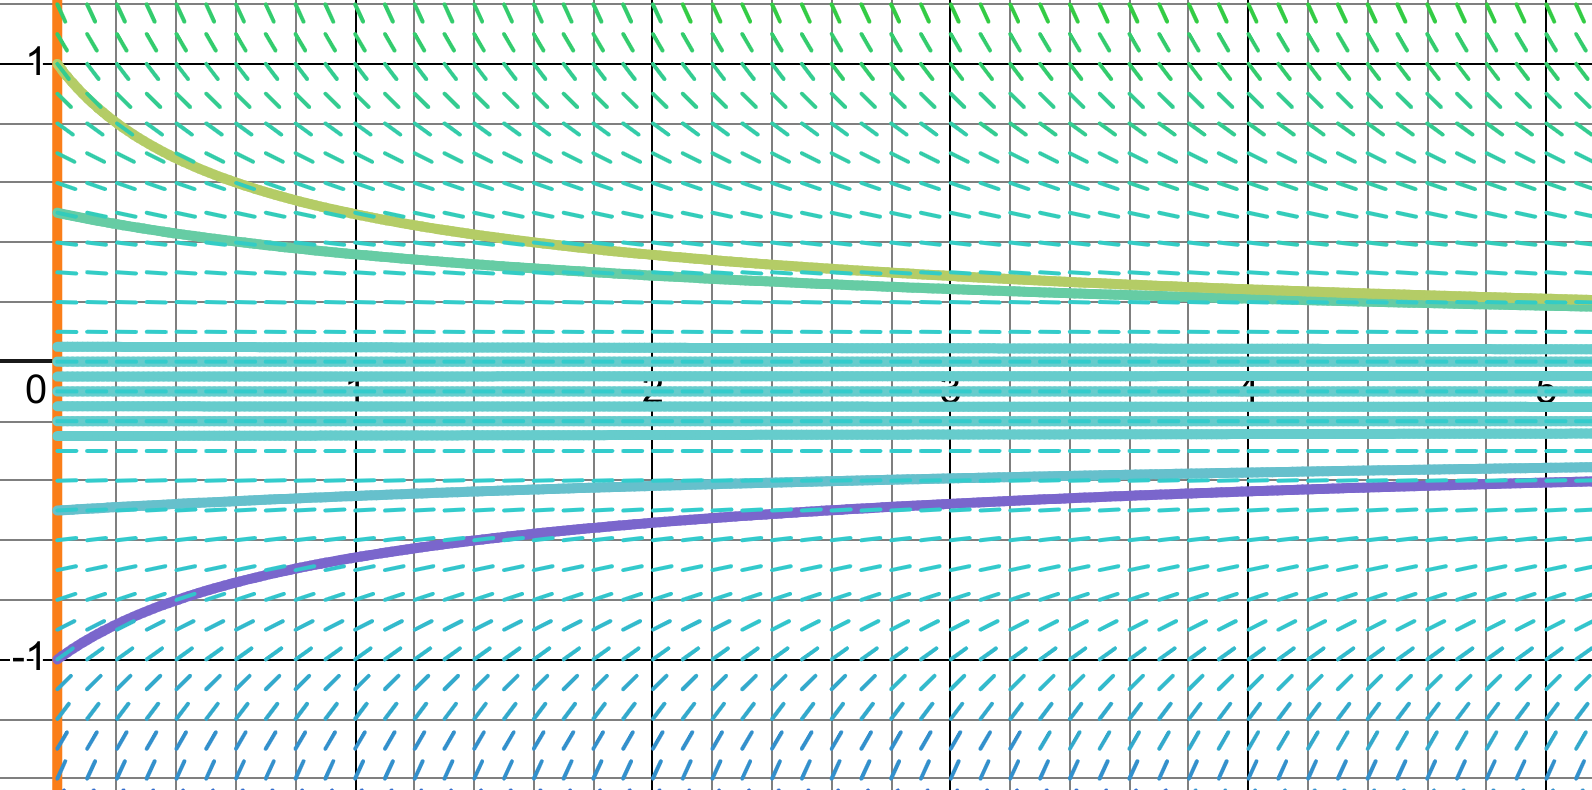
\includegraphics[width=2.5in]{slope-field-ambiguous.png}
	\end{center}


	\bigskip	
	\bigskip	
	\bigskip	
	\begin{parts}
		\item Find all equilibrium solutions.
		\item Use linear approximations to classify the equilibrium solutions as stable/unstable/etc..
	\end{parts}
\end{slide}

\begin{slide}
	\question
	To make a 1d affine approximation of a function $f$ at the point $E$ we have the formula
	\[
		f(x)\qquad \approx\qquad f(E) + f'(E)(x-E).
	\]		

	To make a 2d approximation of a function $\vec F(x,y)=\Big(F_1(x,y), F_2(x,y)\Big)$ at the point $\vec E$,
	we have a similar formula
	\[
		\vec F(x,y)\qquad \approx \qquad \vec F(\vec E) + D_{\vec F}(\vec E)\Big((x,y)-\vec E\Big)
	\]
	where $D_{\vec F}(\vec E)$ is the \emph{total derivative} of $\vec F$ at $\vec E$, which can be expressed
	as the matrix
	\[
		D_{\vec F}(\vec E) = \mat{
			\rule[-0.5cm]{0pt}{.8cm}\displaystyle \frac{\partial F_1}{\partial x} &\displaystyle  \frac{\partial F_1}{\partial y}\\
			\rule[-0.2cm]{0pt}{.3cm}\displaystyle  \frac{\partial F_2}{\partial x} &\displaystyle  \frac{\partial F_2}{\partial y}
		}
	\]
	evaluated at $\vec E$.
\end{slide}

\begin{slide}
	
	Recall our model from Question \ref{q-phase} for the life cycle of a tree where $H(t)$ was
	height, $A(t)$ was the leaves' surface area, and $t$ was time:
	\begin{align*}
		H'(t) &= 0.3\cdot A(t)-b\cdot H(t)\\
		A'(t) &= -0.3\cdot (H(t))^2 + A(t)
	\end{align*}
	with $0 \leq b \leq 2$

	\bigskip
	
	We know the following:
	\begin{itemize}
		\item The equations cannot be written in matrix form.
		\item The equilibrium points are $(0,0)$ and $\Big(\frac{100}{9}b,\frac{1000}{27}b^2\Big)$.			
	\end{itemize}	

	We want to find an affine approximation to the system.

	Define $\vec F(H,A)=(H', A')$
	\begin{parts}
		\item Find the matrix for $D_{\vec F}$, the total derivative of $\vec F$.
		\item Create an affine approximation to $\vec F$ around $(0,0)$ and use this to write an approximation to the original system.
		\item\label{affine-approx}
		 Create an affine approximation to $\vec F$ around $(\frac{100}{9}b,\frac{1000}{27}b^2)$ and use this to write an approximation to the original system.
		
		\bigskip 
		\item Make a phase portrait for the original system and your approximation from part \ref{affine-approx}. How do they compare?
		\item Analyze the nature of the equilibrium solution in part \ref{affine-approx} using eigen techniques. Relate your analysis to
		the original system.

	\end{parts}
\end{slide}

%
% Hours 27-29
%



\begin{bookonly}
%\begin{appendix}\label{APPSLEI}
%	\Title{Systems of Linear Equations I}
%
%	In this appendix you will learn
%	\begin{itemize}
%		\item What a system of linear equations is.
%		\item What the solution set to a system of equations is, and what it means for a system of equations
%			to be consistent or inconsistent.
%		\item How augmented matrices can be used to solve systems of linear equations.
%		\item How to apply row reduction to find a unique solution to a system of linear
%			equations and to determine if a system of linear equations is consistent or inconsistent.
%	\end{itemize}
%
%	\input{modules/appendix1.tex}
%	\input{modules/appendix1-exercises.tex}
%\end{appendix}
%
%
%
%
%\begin{appendix}
%	\PrintExerciseSolutions
%\end{appendix}
	\begin{indices}*
		\Title{Indices}

		\printindex[symbols]

		\bigskip
		\printindex

		\bigskip
		\printindex[definitions]
	\end{indices}
\end{bookonly}

\end{document}
